\chapter{State of the Art: Model Watermarking, Fingerprinting and Attacks}
\label{ch:sota}

%In order to prove ownership the watermarking method has to have a low false positive rate. Suppose that we allow at most $\Delta$ misclassifications among $N$ trigger images. Assuming independence between the classification of each trigger image, we can calculate the probability of successful watermark verification by
%\begin{align*}
%    \mathrm{Pr} = \sum_{\delta = 0}^{\Delta} \begin{pmatrix} N \\ \delta
%    \end{pmatrix} (1-\rho)^{\delta}\rho^{N-\delta},
%\end{align*}
%with $\rho$ being the accuracy of the model on the trigger set \cite{guo_evolutionary_2019, rouhani_deepsigns_2019, guo_watermarking_2018}.

% Isabell: nicht low false negative rate?
% Rudi: Ja, ein false positive hält einen nicht davon ab, ownership zu zeigen. Eigentlich ist es aber wohl besser zu sagen, dass beides niedrig sein muss. Weil wenn ich nur TN niedrig haben will und das ausreicht, kann man einen sehr trivialen detector bauen, der immer richtig ist...

There are several connotations of watermarking, and generally, information hiding, along the machine learning process, as depicted in \cref{fig:watermarking-ml-process}.
% TODO: There was another paper with a similiar idea
Sablayrolles et al. \cite{sablayrolles_radioactive_2020} propose a technique that \textit{traces data usage}; it marks (training) data in a special way, so that a ML model trained on that data will bear a watermark that can be identified  (cf. \circled{1} in \cref{fig:watermarking-ml-process}).
The main body of work, and the focus of this section, consider ML models as the objects that need protection and in which the watermark is embedded  (cf. \circled{2} in \cref{fig:watermarking-ml-process}).
Abdelnabi et al. \cite{abdelnabi_adversarial_2020} propose a special form of watermarking. Their scheme is not watermarking a \textit{model}, but the \textit{output} of a text generating model (cf. \circled{3} in \cref{fig:watermarking-ml-process}). They assume that an attacker could use the model for generating whole articles. In such a case, the watermark can be extracted from the generated text and prove the illegitimate usage of the model.
In some settings, it is further considered that a marked output (prediction, or data) is generated with the explicit goal to trace the usage of this data, e.g. for training by an attacker (cf. \circled{4} in \cref{fig:watermarking-ml-process}). This is a special form of \circled{1}, as the data origin is different, and of \circled{2}, as the adversary model is \textit{implicitly marked} (cf. %. Most methods following this approach are described in 
\cref{sec:wm:countering_extraction}).

We want to point out that information hiding techniques for ML models may have other applications than watermarking. For instance, Song et al. \cite{song_machine_2017} propose a technique to hide data from a private training dataset in the internals of a model (e.g. the weights) trained upon said dataset. 
This way, an attacker that does not have direct access to the training data, but can only let their model be trained on the data by the data owner, can exfiltrate this data via the derived machine learning model, i.e. perform a data exfiltration attack  (cf. \circled{5} in \cref{fig:watermarking-ml-process}).
We, however, consider techniques which hide information about a lawful owner of the model. 
\begin{figure}
\centering
    % ------ ML process overview figure

\begin{tikzpicture}
\node[inner sep=0pt] (mlProcess) at (-2.1,0) {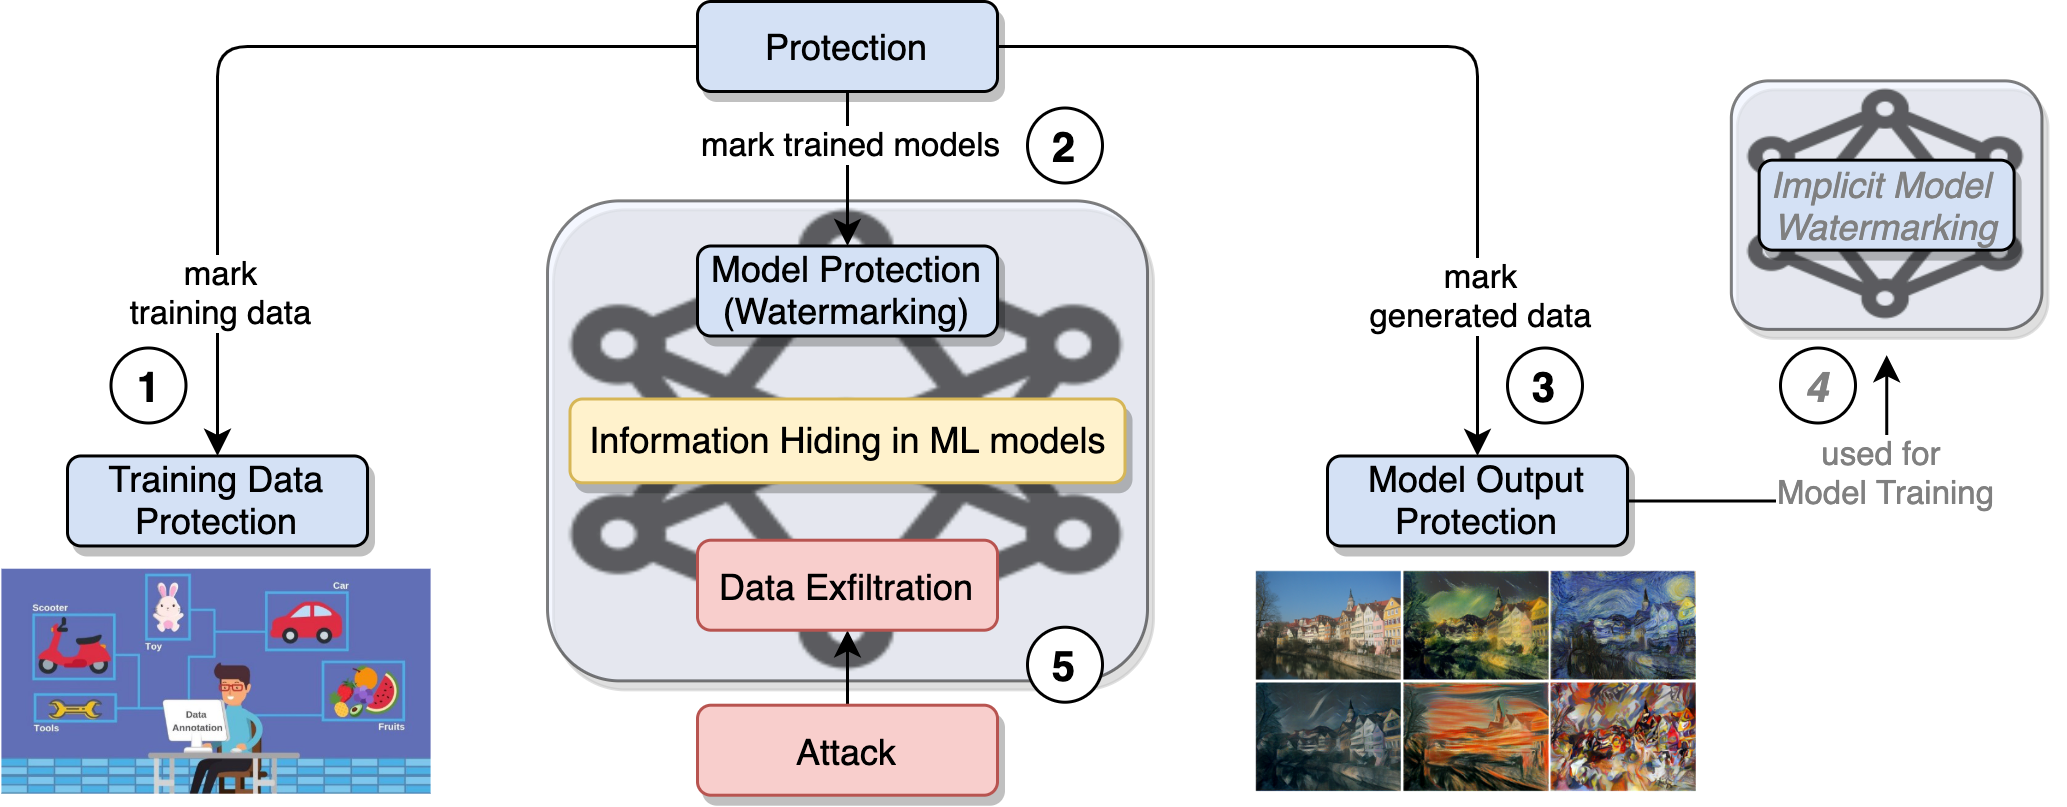
\includegraphics[width=\linewidth]{images/Watermarking_aspects.png}};

%MarkTrainingData:
\node[inner sep=0pt] (cite200) at (-7.5,0.1) {\tiny \cite{sablayrolles_radioactive_2020}};
%MarkOutputData:
% marks output, doesn't talk about model training
\node[inner sep=0pt] (cite211) at (0.7,0.1) {\tiny \cite{abdelnabi_adversarial_2020}};

%specifically for model training!
\node[inner sep=0pt] (cite212) at (4.5,0.35) {\tiny \cite{szyller_dawn_2020}};

% marks all output for surrogate model training
\node[inner sep=0pt] (cite213) at (4.5,0.1) {\tiny \cite{zhang_model_2020}};
\node[inner sep=0pt] (cite214) at (4.5,-0.15) {\tiny \cite{wu_watermarking_2020}};
%OtherInformationHiding
\node[inner sep=0pt] (cite225) at (-2.5,-1.8) {\tiny \cite{song_machine_2017}};
\end{tikzpicture}
    \caption{Different notions of information hiding along a ML process}
    \label{fig:watermarking-ml-process}
\end{figure}

The vast majority of watermarking methods for ML models is designed specifically for DNNs. The main reason for this is not only the high value of DNNs, as they require large datasets and long training time, but also the number of "degrees of freedom" in a DNN. Large DNNs thus have, compared to other ML models, more "space" for hiding marks. 
Most authors evaluate the schemes on image classification task. However, some authors extend the methods to other tasks, like audio classification \cite{jia_entangled_2020}, image captioning \cite{lim_protect_2020}, image processing \cite{quan_watermarking_2020, wu_watermarking_2020, zhang_model_2020} (where the output is an image/data, rather than a prediction), or specific learning settings, such as GANs \cite{skripniuk_black-box_2020}, Federated Learning with DNNs \cite{atli_waffle_2020},
%\footnote{Preceding master thesis in \cite{xia_watermarking_2020}}
Graph Neural Networks \cite{zhao_watermarking_2020}, and Deep Reinforcement Learning \cite{behzadan_sequential_2019}.

\section{Requirements} \label{sec:requirements}
A watermarking scheme should fulfil a couple of requirements. Literature is not coherent in the naming of these requirements of watermarking (and fingerprinting) methods, and we, therefore, aim at providing a common nomenclature. 
To this end, we collect all the requirements that were proposed in the papers included in our literature review and list them in \cref{tab:requirement}, identifying also terms used as synonyms, along with references to the respective publications.

\begin{table*}[t]
\centering
% No punctuation in last sentence + caption should be set as an inverted pyramid. see IEEE editorial style manual: http://journals.ieeeauthorcenter.ieee.org/wp-content/uploads/sites/7/IEEE-Editorial-Style-Manual_081920.pdf
\caption{Requirements for Watermarking techniques. The notation is not consistent throughout the papers, but the terms in the left column are the most prominent ones. These requirements mostly apply also to Fingerprinting methods}
%  \begin{adjustbox}{width=1.0\textwidth,center=\textwidth}

\rowcolors{2}{gray!15}{white}

\begin{tabular}{|p{0.15\textwidth}|p{0.4\textwidth}|p{0.4\textwidth}|}
\rowcolor{gray!15}
\hline
\textbf{Property}               & \textbf{Description}                                                                                              & \textbf{Other terms used in papers}                        \\ \hline
%
Effectiveness                   & The model owner should be able to prove ownerhsip anytime and multiple times if needed                            & Authentication \cite{li_piracy_2020}, Functionality \cite{li_how_2019}                              \\ \hline
%
Fidelity                        & The accuracy of the model should not be degraded after embedding the watermark                                    & Funcionality-preserving \cite{li_piracy_2020, wang_robust_2020, adi_turning_2018}, Loyalty \cite{merrer_adversarial_2019}, Utility \cite{szyller_dawn_2020}
\scriptsize{(Image WM: Transparency \cite{potdar_survey_2005}; Relational Data WM: Usability \cite{kamran_comprehensive_2018})}                \\ \hline
%
Robustness                      & The embedded watermark should resist a designated class of transformations                                        & Unremovability \cite{adi_turning_2018, szyller_dawn_2020}                                            \\ \hline
%
Security                        & The watermark should be secure against brute-force or specifically crafted evasion attacks                        & Secrecy \cite{skripniuk_black-box_2020}, Unforgeability \cite{adi_turning_2018, wang_robust_2020}                                    \\ \hline
%
Legality                        & An adversary cannot produce a watermark for a model that was already watermarked by the model owner               & Ownership piracy resilient \cite{adi_turning_2018, wang_robust_2020}, Non-ownership piracy \cite{szyller_dawn_2020}           \\ \hline
%
Integrity                       & The watermark verification process should have a negligible false positive rate                                   & Low false positive rate \cite{guo_evolutionary_2019, guo_watermarking_2018}, Non-trivial ownership \cite{li_piracy_2020, adi_turning_2018, wang_robust_2020}, Uniqueness \cite{quan_watermarking_2020} \\ \hline
%
Reliability                     & The watermark verification process should have a negligible false negative rate                                   & Credibility \cite{chen_blackmarks_2019}                                                \\ \hline
%
Efficiency                      & The watermarking embedding and verification process should be fast                                                &                                                            \\ \hline
%
Capacity                        & The watermarking scheme should be capable of embedding a large amount of information                              & Payload \cite{guo_watermarking_2018}                                                    \\ \hline
%


% \hline
% \textbf{Property}     & \textbf{Description}                                                                                    & \textbf{Other terms used in papers}                        \\ \hline
% Fidelity              & The accuracy of the model should not be degraded after embedding the watermark                          & Funcionality-preserving \cite{li_piracy_2020, wang_robust_2020, adi_turning_2018}, Loyalty \cite{merrer_adversarial_2019}, Utility \cite{szyller_dawn_2020}
% \scriptsize{(Image WM: Transparency \cite{potdar_survey_2005}; Relational Data WM: Usability \cite{agostino_cortesi_watermarking_2010})}       \\ \hline
% Robustness            & The embedded watermark should resist a designated class of transformations                        & Feasibility \cite{li_how_2019}                                      \\ \hline
% Non-trivial ownership & An adversary should not be able to claim ownership of the watermarked model without knowing the watermark        &                                                  \\ \hline
% Legality              & An adversary cannot produce a watermark for a model that was already watermarked by the model owner                        & Ownership piracy resilient \cite{adi_turning_2018}, non-ownership piracy \cite{szyller_dawn_2020} \\ \hline
% Reliability           & The watermark verification process should have a negligible false negative rate                         & Credibility \cite{chen_blackmarks_2019}                               \\ \hline
% Integrity             & The watermark verification process should have a negligible false positive rate                         & Low false positive rate \cite{guo_evolutionary_2019, guo_watermarking_2018}  \\ \hline
% Capacity              & The watermarking scheme should be capable of embedding a large amount of information                  & Payload \cite{guo_watermarking_2018}                                     \\ \hline
% Efficiency            & The watermarking embedding and verification process should be fast &                                                  \\ \hline
% Effectiveness         & The model owner should be able to prove ownerhsip anytime and multiple times if needed                                                                  & Authentication \cite{li_piracy_2020}                                   \\ \hline
% Security              & The watermark should be secure against brute-force or specifically crafted evasion attacks                                  & Unremovability \cite{szyller_dawn_2020, adi_turning_2018}                             \\ \hline


\end{tabular}
% \end{adjustbox}
\label{tab:requirement}
\end{table*}

%TODO? Tamper-resistance?
%Tamper resistance:  Tamper-detection watermarking was developed to check the authenticity of digital photographs.  Watermarks of  this  type  are  sensitive  to  any change of  the content data;  thus,  by  checking  the integrity  of the  watermark,  the  system  can  determine whether or not the content has the ever been modified or replaced
 

The most important %and obvious 
requirements are  \textbf{effectiveness}: the watermark shall be embedded in a way that the model owner can prove ownership anytime, \textbf{fidelity}: the model's accuracy shall not be degraded because of the watermark embedding, and \textbf{robustness}: the watermark embedding should be robust against several kinds of attacks, including fine-tuning, model compression and other, specifically crafted attacks.
%
The remaining requirements are listed in \cref{tab:requirement}. 
% Other important requirements are \textbf{security}: the watermark shall be secure against brute-force and evasion attacks,  \textbf{legality}: the adversary shall not be able to watermark an already watermarked model, \textbf{integrity}: the watermark embedding shall yield to minimal false positive rate, \textbf{reliability}: the watermark embedding shall yield to a minimal false negative rate, \textbf{efficiency}: the watermarking scheme shall have a minimal overhead, \textbf{capacity}: the watermark should be able to carry a lot of information.
% end candidate for deletion
Note, that non-trivial ownership is sometimes used as a synonym for integrity, meaning that innocent models are not being accused of ownership piracy, but also as a requirement that an attacker cannot easily claim ownership without knowing the watermarking scheme and embedded watermark. Moreover, authentication is more a subset of effectiveness than a real synonym since it only requires that there is a provable association between an owner and their watermark. \textbf{Feasibility} is used as a combination of robustness and effectiveness \cite{li_how_2019}, and \textbf{correctness} as a combination of effectiveness, reliability, and integrity \cite{lukas_deep_2020}. Fingerprinting should fulfil two more requirements: \textbf{uniqueness} -- the fingerprint can be uniquely identified with the user, and \textbf{scalability} -- the fingerprinting scheme should be able to embed multiple fingerprints, either in the same model or in multiple versions of the model. A fingerprinting method that embeds multiple fingerprints, e.g. \cite{chen_deepmarks_2019}, could not only trace back the attacker but also identify collaboration between several malicious users.
 
\begin{sidewaystable}
    \centering

\caption{Requirements met by watermarking and fingerprinting schemes.  We distinguish two degrees:
%$\sim$ indicates a claim -- the authors of the scheme claim that the scheme fulfils this property; \checkmark indicates a demonstration -- the authors show empirically that the property is fulfilled
$\sim$ indicates: the respective authors claim the scheme fulfils this property; \checkmark indicates: the authors show empirically that the property is fulfilled
}

\rowcolors{2}{white}{gray!15}

\setlength\tabcolsep{2pt}
\setlength\extrarowheight{5pt}

\begin{tabular}{|l|c|c|c|c|c|c|c|c|c|c|c|c|c|c|c|c|c|c|c|c|c|c|c|c|c|c|c|c|c|c|c|}
\rowcolor{gray!15}
\hline
 & \multicolumn{7}{l|}{\textbf{white-box}}                                                                             & \multicolumn{24}{l|}{\textbf{black-box}}                                                                                                                                                                                                                                                                                                                                                                 \\ \cline{2-32} 
%                                     & \multicolumn{2}{l|}{\textbf{into pdf}} & \multicolumn{4}{l|}{\textbf{into weights}}                   & \textbf{?} & \textbf{OOD, pattern, noise} & \textbf{OOD} & \textbf{pattern} & \textbf{}         &                   &        & \multicolumn{5}{l|}{\textbf{perturbation}}           & \textbf{in-distr} & \multicolumn{2}{l|}{\textbf{aginst ME}} & \multicolumn{3}{l|}{\textbf{labels}} & \multicolumn{4}{l|}{\textbf{extending existing work}}          & \multicolumn{3}{l|}{\textbf{image processing}}            \\ \hline
%
\hline
\multicolumn{1}{|l|}{\textbf{Property}}      & {\tiny\cite{rouhani_deepsigns_2019}}         & {\tiny\cite{chen_deepmarks_2019}}      & {\tiny\cite{uchida_embedding_2017}}     & {\tiny\cite{wang_robust_2020}} & {\tiny\cite{wang_watermarking_2020}} & {\tiny\cite{feng_watermarking_2020}}       & {\tiny\cite{chen_specmark_2020}}   & {\tiny\cite{zhang_protecting_2018}}                        & {\tiny\cite{adi_turning_2018}}          & {\tiny\cite{li_piracy_2020}}       & {\tiny\cite{guo_watermarking_2018}} & {\tiny\cite{guo_evolutionary_2019}} & {\tiny\cite{zhu_secure_2020}}    & {\tiny\cite{merrer_adversarial_2019}} & {\tiny\cite{li_how_2019}} & {\tiny\cite{chen_blackmarks_2019}}  & {\tiny\cite{zhao_afa_2019}} & {\tiny\cite{lukas_deep_2020}} & {\tiny\cite{namba_robust_2019}}             & {\tiny\cite{szyller_dawn_2020}}       & {\tiny\cite{jia_entangled_2020}}                     & {\tiny\cite{zhong_protecting_2020}}     & {\tiny\cite{zhang_deeptrigger_2020}}    & {\tiny\cite{xu_identity_2020}}      & {\tiny\cite{yang_effectiveness_2019}}      & {\tiny\cite{guan_reversible_2020}} & {\tiny\cite{skripniuk_black-box_2020}} & {\tiny\cite{lim_protect_2020}} & {\tiny\cite{wu_watermarking_2020}}       & {\tiny\cite{zhang_model_2020}} & {\tiny\cite{quan_watermarking_2020}}       \\ \hline
\multicolumn{1}{|l|}{Effectiveness} & \checkmark      & \checkmark                 & \checkmark & \checkmark   &  \checkmark                   & \checkmark & \checkmark           & \checkmark                   & \checkmark   & \checkmark             & \checkmark              & \checkmark              & \checkmark   & \checkmark   & \checkmark    &   \checkmark          & \checkmark      & \checkmark    & \checkmark              & \checkmark          & \checkmark                    & \checkmark      & \checkmark           & \checkmark    & \checkmark      & \checkmark             & \checkmark             & \checkmark   & \checkmark             & \checkmark                &  \checkmark \\ \hline
\multicolumn{1}{|l|}{Fidelity}      & \checkmark            & \checkmark                 & \checkmark       & \checkmark         & \checkmark                & \checkmark       & \checkmark       & \checkmark                         & \checkmark         & \checkmark             & \checkmark              & \checkmark              & \checkmark   & \checkmark   & \checkmark    & \checkmark        & \checkmark   & \checkmark & \checkmark              & \checkmark          & \checkmark                    & \checkmark      & \checkmark           & \checkmark    & \checkmark      & \checkmark             & \checkmark             & \checkmark         & \checkmark                   &                     & \checkmark       \\ \hline
% \multicolumn{1}{|l|}{Robustness}    & FT, MC, OW      & FT, MC, OW           & FT, MC     & FT, MC, OW   & FT, MC              & FT, MC, OW & FT, MC, TL & FT, MC                       & FT, TL       & FT, MC           & $\sim$             & FT                & FA, TL & FT, MC & FT      & FT, MC , OW & FT, MC    & \checkmark    & FT, MC            & ME            & ME, MC, FT, NC, FP       & FT, MC    & FT, MC, OW     & MC      & FT, MC, D &                  & FT,  MC          & FT, MC       & cropping, adding noise & \checkmark                & FT, MC, OW \\ \hline
\multicolumn{1}{|l|}{Robustness}    & \checkmark & \checkmark & \checkmark & \checkmark & \checkmark & \checkmark & \checkmark & \checkmark & \checkmark & \checkmark & $\sim$ & \checkmark & \checkmark & \checkmark & \checkmark     & \checkmark & \checkmark & \checkmark    & \checkmark  & \checkmark  & \checkmark  & \checkmark & \checkmark  & \checkmark & \checkmark &                  & \checkmark & \checkmark & \checkmark & \checkmark & \checkmark \\ \hline
\multicolumn{1}{|l|}{Security}      & \checkmark            & \checkmark                 & $\sim$      & $\sim$        & $\sim$               &            & $\sim$      & \checkmark                         & $\sim$        &                  & \checkmark              &                   & \checkmark   & $\sim$  & \checkmark    & \checkmark        &           &         &                   &               &                         &           & \checkmark           &         &           &                  & \checkmark             &              & \checkmark                   &                     &            \\ \hline
\multicolumn{1}{|l|}{Legality}      &                 &                      &            & $\sim$        &                     &            &            &                              &              &                  &                   &                   &        &        & \checkmark    &             &           &         &                   & $\sim$         &                         &           &                &         &           &                  &                  &              &                        &                     &            \\ \hline
\multicolumn{1}{|l|}{Integrity}     & \checkmark            & \checkmark                 &            & \checkmark         &                     &            & \checkmark       &                              & \checkmark         & \checkmark             & \checkmark              & \checkmark              &        &        & \checkmark    & \checkmark        & \checkmark      & \checkmark    &                   &               &                         &           & \checkmark           &         &           &                  &                  &              &                        &                     &            \\ \hline
\multicolumn{1}{|l|}{Reliability}   & \checkmark            & \checkmark                 &            &              &                     &            & $\sim$      &                              &              &                  &                   &                   &        &        &         & \checkmark        & \checkmark      & \checkmark    &                   & \checkmark          &                         &           &                &         &           &                  &                  &              &                        &                     &            \\ \hline
\multicolumn{1}{|l|}{Efficiency}    & \checkmark            & \checkmark                 & $\sim$      &              & $\sim$               & \checkmark       & \checkmark       &                              &              &                  &                   &                   &        & $\sim$  &         & \checkmark        &           &         &                   & \checkmark          &                         & \checkmark      &                &         &           &                  &                  &              &                        &                     &            \\ \hline
\multicolumn{1}{|l|}{Capacity}      & \checkmark            &                      & \checkmark       &              & \checkmark                & \checkmark       &            &                              &              &                  & \checkmark              &                   &        &        &         & \checkmark        &           &         &                   &               &                         &           &                &         &           &                  & \checkmark             & \checkmark         & \checkmark                   &                     & $\sim$      \\ \hline
\end{tabular}

\label{tab:summary-req}

\end{sidewaystable}







We provide an overview of all the watermarking and fingerprinting schemes considered in this thesis, and whether they are meeting the above-mentioned requirements, in \cref{tab:summary-req}.
%, which is inspired by \cite{li_how_2019}. We extend their summary by incorporating the additional identified requirements, and from their initially considered seven schemes to the XX schemes investigated in this paper.
%TODO: describe what we can learn from this table.
We observe %from \cref{tab:summary-req} 
that all schemes fulfil the above-identified most important requirements of fidelity, effectiveness and integrity, except for \cite{guan_reversible_2020}, which on purpose gives up on robustness in favour of reversibility: the authors point out that the application of their scheme is not IPP, but integrity authentication, and that all existing watermarking methods are irreversible -- once the watermark is embedded, it cannot be removed to restore the original model without degrading the model's performance.
They argue that irreversible watermarking schemes are permanently modifying the model's internals, and thus destroying the integrity of the model, which could have severe consequences especially in applications for the medical or defence domain, etc.
%Therefore, the authors introduce the first reversible black-box watermarking scheme.
To make the scheme reversible they sacrifice the robustness requirement, inspired by traditional image integrity. % and Guan et al. adapted it to DNNs.
For Zhang et al.'s method \cite{zhang_model_2020}, the fidelity requirement does not apply since it is not well-defined for image processing. To determine for a model that outputs an image (or other complex data) whether a watermarked version of such a model is comparable to the original one, one would need to define a similarity measure to compare if the two outputs are equivalent.

Watermarking methods can be categorised into two main fields, \textit{white-box} and \textit{black-box} watermarking. White-box means that the model owner needs access to the stolen model's parameters or other model characteristics, in either step of the IPP method process, i.e. also during watermark extraction and verification. A black-box method generally only needs access to the model's prediction, e.g. via an API service, to observe matching input and output from the ML model, using it in a similar fashion as an \textit{oracle}. In the following sections, we discuss both of the watermarking types.

\begin{figure}
     \centering
     \begin{subfigure}[b]{0.7\textwidth}
         \centering
         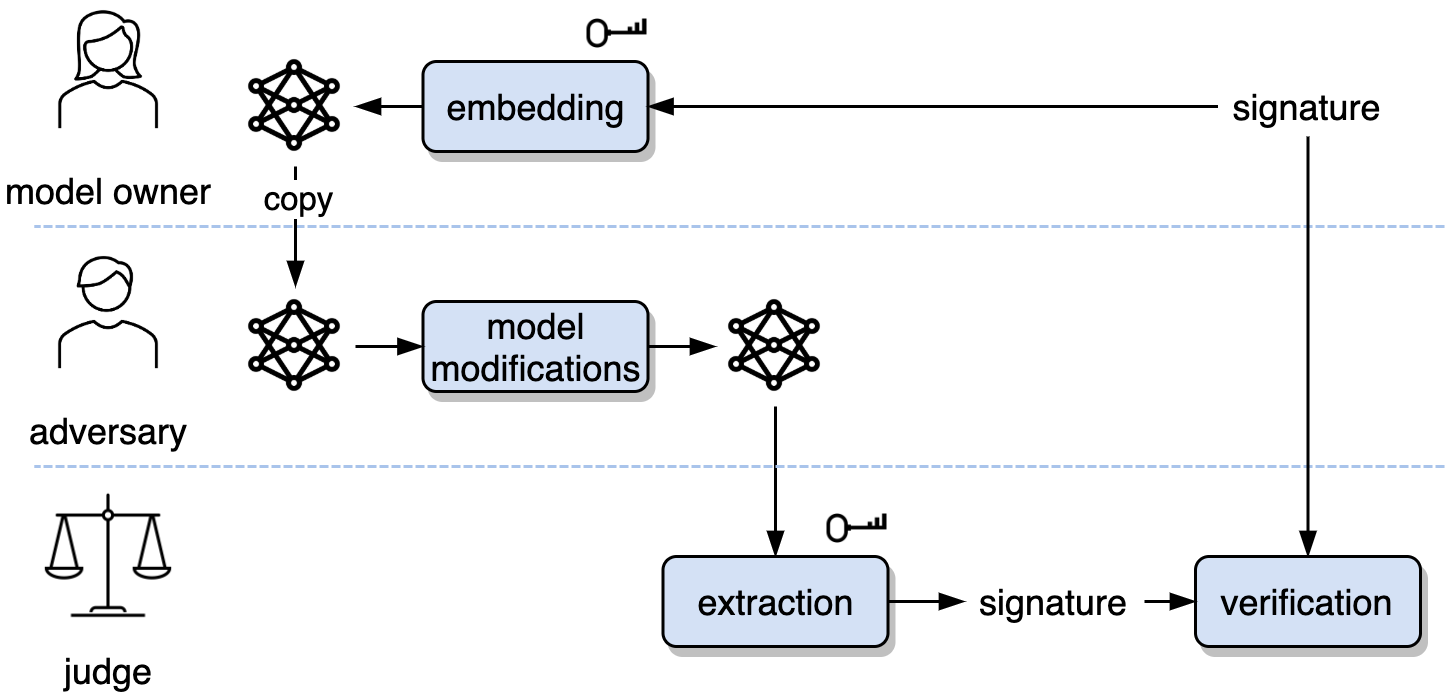
\includegraphics[width=\textwidth]{images/whitebox_workflow.png}
         \caption{}
         \label{fig:whitebox-workflow}
     \end{subfigure}
     \hfill
     \begin{subfigure}[b]{0.7\textwidth}
         \centering
         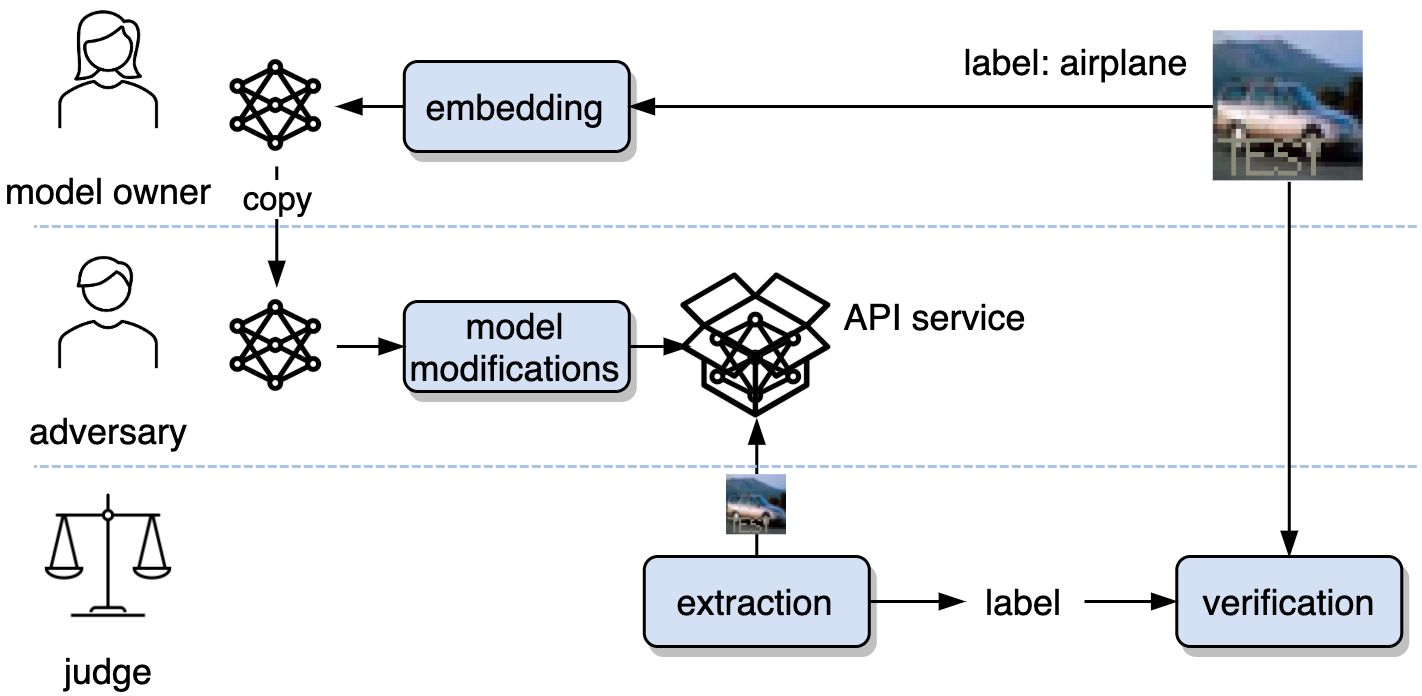
\includegraphics[width=\textwidth]{images/blackbox_workflow.png}
         \caption{}
         \label{fig:blackbox-workflow}
     \end{subfigure}
        \caption{Typical workflows for (a) white-box watermarking and (b) black-box watermarking}
        \label{fig:bothworkflows}
\end{figure}

\section{White-box Watermarking}
\label{sec:whitebox}
White-box watermarking requires full access to the model in order to verify the watermark. Usually, the model owner creates a $T$-bit signature vector $\mathbf{b} \in \{0,1\}^T$ that is a set of arbitrary binary strings that should be independently and identically distributed (iid) \cite{rouhani_deepsigns_2019}. This binary vector serves as a watermark and is usually embedded into the model by fine-tuning with regularisation. We call this type of embedding scheme \textit{regulariser based}. The general workflow for a regulariser based embedding scheme is illustrated in \cref{fig:whitebox-workflow}.

% --- regulariser based - into weights --- fingerprinting potential
The first framework for embedding a watermark into a DNN was proposed by Uchida et al. \cite{uchida_embedding_2017}\footnote{Slightly extended version in \cite{nagai_digital_2018}} in 2017. They follow the idea of embedding a signature into the model, particularly in the DNN's weights. 
While it would be possible to directly alter the model's parameters, as it would be done for watermarking relational data, this would degrade the model's performance.
%They point out that it would be possible to directly change the model's parameters but this would degrade the model's performance as they show experimentally and thus propose embedding the watermark while training the network. Furthermore, t
They thus describe three ways of embedding the watermark: while training, while fine-tuning, or by using the distilling approach \cite{hinton_distilling_2015}. The fine-tuning approach is especially interesting when the model owner wants to place individual watermarks (i.e. fingerprints) before distributing to different users, in order to trace back the recipient in case of copyright infringement (cf. \cref{sec:fingerprinting:user-specific-wm}). The model is trained with a regulariser term, given the signature $\mathbf{b} \in \mathbb{R}^T$, the averaged weights vector $\mathbf{w} \in \mathbb{R}^M$ and a specially crafted \textit{embedding matrix} $\mathbf{M} \in \mathbb{R}^{T \times M}$. The embedding matrix $\mathbf{M}$ can be considered a secret key for the embedding and extracting process. The watermark is extracted by applying $\mathbf{M} \in \mathbb{R}^{T \times M}$ to the weights vector $\mathbf{w} \in \mathbb{R}^M$ and then applying a step function:
\begin{align}
    \mathbf{\tilde b}_j = s(\sum_{i=1}^M \mathbf{M}_{ji}\mathbf{w}_i),
\end{align}
where $s(\cdot)$ is the unit step function. The resulting vector $\mathbf{\tilde b}$ is then compared with the signature $\mathbf{b}$ and the BER (bit error rate) is computed. Ownership is proven by thresholding the BER. 
%In watermark extraction, the $T$-bit signature is reconstructed by $\mathbf{b}_j = s(\sum_{i=1}^M \mathbf{M}_{ji}\mathbf{w}_i)$, where $s(\cdot)$ is the unit step function. 
%Besides experiments for effectiveness and fidelity, they tested their scheme for robustness against fine-tuning and model compression.
%They showed experimentally that their proposed framework achieved low test error and embedding loss $\mathcal{L}_R$ in all three of the above mentioned embedding situations.

% ---- regulariser based - into pdf ----
Subsequently, Rouhani et al. \cite{rouhani_deepsigns_2019} propose a watermarking framework that proves to be more robust against watermark removal, model modifications and watermark overwriting than \cite{uchida_embedding_2017}.
The method is regulariser based and encodes the signature in the PDF of activation maps obtained at different DNN layers, by
%They formulate two constraints to be considered during DNN training which results in using two additive 
%the use of two regularisation loss functions.
one additional regularisation term $\mathcal{L}_1(w)$ that ensures that selected activations are isolated from other activations, to avoid creating a detectable pattern of alterations and another $\mathcal{L}_2(w)$ to enforce that the distance between the owner-specific WM signature and the transformation of isolated activations is minimal:
%, instead of only one as in \cite{uchida_embedding_2017}.
% They formulate two additional constraint which need to be considered during DNN training in order to embed the watermark: "(i) Selected activations shall be isolated from other activations". "(ii) The distance between the owner-specific WM signature and the transformation of isolated activations shall be minimal". The second constraint is comparable to the only constrained used in \cite{uchida_embedding_2017}.
%The embedding into the model is achieved by fine-tuning with two additive regularisation loss functions, each of these two specific loss functions addressing a constraint:
\begin{align}
    \mathcal{L}(w) = \mathcal{L}_0(w) + \lambda_1 \mathcal{L}_1(w) + \lambda_2 \mathcal{L}_2(w)
 \end{align}
%Furthermore, they propose a black-box way how to verify the regulariser based watermark.
For extraction, they save a list consisting of the selected Gaussian classes, the trigger images and the projection matrix. In the verification process, the trigger images are used as input for the model to then analyse the activations. The scheme can be employed in a white-box or black-box setting, depending on whether just the output layer or also hidden layer activations are assumed to be available in case a watermark verification is needed.
%Info aus \cite{zhang_deeptrigger_2020}:
%Rouhani et al. [21] exploited two loss functions to modify the weights of the model and to produce a specific activation under a particular input. Thus, it works in both white-box and black-box environments.

% ---- GAN-like network but also regulariser based ---
Wang et al. \cite{wang_robust_2020}\footnote{Newer and slightly changed version in \cite{wang_riga_2020}} generalise both of the above presented algorithms into a white-box scheme. They show that the previous schemes are vulnerable to watermark detection (cf. \cref{sec:attacks})%\footnote{Wang et al. present especially attacks on watermarks also in \cite{wang_attacks_2019}%, where they describe the vulnerability of existing white-box watermarking schemes. We will cover that in \cref{sec:attacks}}
, as the weight distribution deviated from those of non-watermarked models. The authors claim that this arises from the additive regularisation loss function(s). Therefore, they propose a new scheme that is particularly robust against detection attacks.
Inspired by the training of GANs, they train a watermarked target DNN $\mathcal{F}_{tgt}$, which is competing against a detector DNN $\mathcal{F}_{det}$ that aims to discover whether a watermark is embedded.
%The target DNN $\mathcal{F}_{tgt}$ -- from the embedding process resulting watermarked DNN -- is trying to compete against a detector DNN $\mathcal{F}_{det}$, which aims to discover whether a watermark is embedded in $\mathcal{F}_{tgt}$.
%For watermark extraction, another DNN is trained in parallel.% to perform this task.
% note: no attack-paper was published against this method

% --- auch regulariser based
Wang et al. \cite{wang_watermarking_2020} follow a similar approach and propose a white-box scheme for DNNs that makes use of an additional DNN for the watermark embedding process. The target model is trained in parallel with an embedding model%\footnote{The authors call it the independent network}
, which will be kept secret after the embedding process. % and further used for the watermark verification process.
%This scheme is basically a regulariser based scheme and compares itself to \cite{uchida_embedding_2017}.
%The idea is to embed the signature into the weights that converge early.
% In the paper, "a weight is considered as converged if the sample standard deviation of the latest 5 updated values during training is less than a threshold".
%The weights selection can be done either manually or automatically. The selected weights will be then fed into the embedding network. For the automated selection, an additional hidden layer is placed between the input weights from the target model and the embedding model such that this hidden layer has the purpose to choose the weights appropriately. 
%Let denote the loss function for the target model as $L_1$ and the loss function for the embedding network as $L_2$.
%The target model's weights are then updated by back-propagation with the loss $L_1$ and $L_2$, and the embedding model only with $L_2$.
The scheme is regulariser based and the watermark is verified by feeding the selected weights into the embedding model and thresholding the output vector. % This will result in the $T$-bit signature. 
They empirically show that their scheme achieves better fidelity, robustness and capacity compared to \cite{uchida_embedding_2017}.

% ---- binarization and compensation mechanism
Feng et al. \cite{li_watermarking_2020} combine a binarisation scheme and an accuracy compensation mechanism to reduce the model's accuracy degradation that results from fine-tuning. They use spread-spectrum modulation on the signature $\mathbf{b}$ and embedding it in different layers to reduce the risk of the watermarked weights being set to zero during a pruning attack.
%, "so that each bit of it is distributed redundantly in all selected layers to enhance the watermark robustness". %The modulation uses a secret key $K_1$. The selection of the weights for watermarking makes use of a pseudo-random number generator with the second secret key $K_2$.
The binarisation scheme then transforms the selected weights per layer so that the overall energy, i.e. the second norm of the selected weights in one layer remains unchanged. The overall energy is defined as
\begin{align}
||sw^j||_2= \sqrt{\sum_{i = 1}^T (sw_i^j)^2 },
\end{align}
where $sw^j$ is the selected weights vector in the $j$-th layer of the selected layers.
Therefore, the embedding position of the watermark cannot be discovered easily by an attacker.
%With energy they mean the second norm

As the last step, they use a "compensation mechanism" in fine-tuning, which aims to reduce the impact of watermark embedding on the model's performance. In particular, they propose to keep the watermarked weights unchanged and fine-tune only all the other weights.

% ----- Chen: SpecMark:A Spectral Watermarking Framework for IP Protection of Speech Recognition Systems
The first (and so far only) white-box framework for Automatic Speech Recognition (ASR) was introduced by Chen et al. \cite{chen_specmark_2020}, called \textit{SpecMark}. The framework embeds the watermark in the spread spectrum of the ASR model without re-training it. They evaluate \textit{SpecMark} on the DeepSpeech model and conclude that it does not have any impact on fidelity.
% -> hat (noch?) keine Einteilung in IPP_overview

\section{Black-box Watermarking}
\label{sec:blackbox}
Black-box watermarking only needs access to the model outputs for watermark verification, which makes watermark verification far more practical. A typical workflow %of a black-box watermarking framework 
is shown in \cref{fig:blackbox-workflow}.

Only two of the existing black-box watermarking frameworks \cite{jia_entangled_2020, szyller_dawn_2020} address the second threat model case (illegal copy) in \cref{sec:threatmodel}. All the other watermarking methods are not reliably robust against model extraction attacks, and therefore primarily address the first case (legal copy).
%We start discussing the methods for the first threat model case.

All of the frameworks that are defending against the legal copy case utilise \textit{(defensive) backdooring}. A \textit{backdoor} consists of a so-called \textit{trigger set} of input-output pairs, which are only known to the backdoor creator (in most cases, the model owner), and triggers a behaviour that is not predictable by others. We call the input images of the trigger set \textit{trigger images}, sometimes \textit{watermarks}, and the corresponding labels \textit{trigger labels}.

Existing black-box watermarking methods concentrate on either creating suitable trigger images (inputs) or trigger labels. Depending on the scheme, different trigger images are used for watermarking:
\begin{itemize}
    \item \textbf{Out-of-distribution (OOD)} trigger images are completely unrelated to the dataset, e.g. abstract images in a handwritten digit dataset.
    \item \textbf{In-distribution} trigger images are taken from the original training dataset and re-labelled wrongly.
    \item \textbf{Pattern based} trigger images originate from the training dataset but are marked with a pattern, e.g. logo, text or other designed pattern -- comparable to patterns embedded in images for "conventional" data poisoning attacks (e.g. \cite{gu_badnets_2019}).
    \item \textbf{Noise based} trigger images are images from the training dataset with added noise (i.e. no systematic pattern), either visible or invisible to the human eye.
    \item \textbf{Perturbation based} trigger images are slightly perturbed images and lie near the classification boundary, thus when re-labelled, they force the model to slightly shift its classification boundary.
\end{itemize}

\cref{fig:blackbox} shows examples for all these five types of trigger images. 
Similar to embedding backdoors %into classifiers for other purposes (generally
as an attack to reduce the availability or integrity of a model, the main objective is that the model will accurately behave on the main classification task, but will fail the classification on the trigger images in the way the model owner has designated.

% --- trigger images figure ----
\begin{figure*}[t]
        \centering
  \subfloat[Out-of-distr. \cite{adi_turning_2018}\label{fig:trigger-a}]{%
       
\includegraphics[height = 2.3cm]{images/weakness/Adi-031.png}}
        \hfill
    \subfloat[In-distr. \cite{namba_robust_2019}\label{fig:trigger-b}]{%
        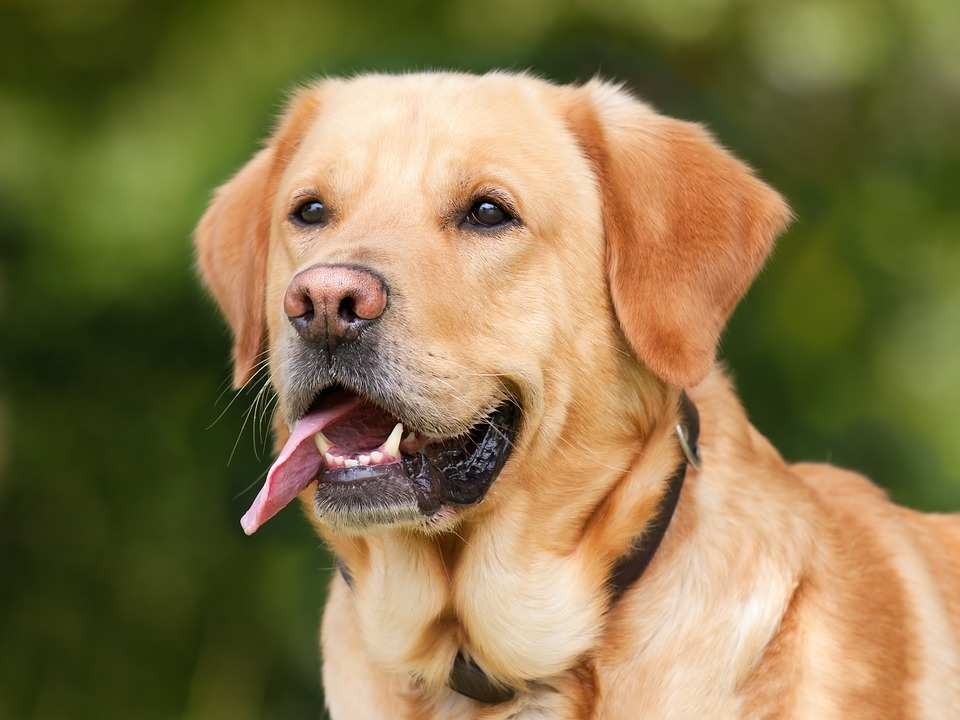
\includegraphics[height = 2.3cm]{images/weakness/Adi-003.png}}
    \hfill
  \subfloat[Pattern \cite{zhang_protecting_2018}\label{fig:trigger-c}]{%
       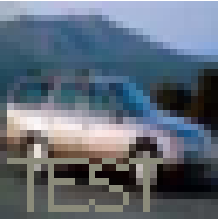
\includegraphics[height = 2.3cm]{images/protecting/Zhang-034.png}}
    \hfill
  \subfloat[Noise \cite{zhang_protecting_2018}\label{fig:trigger-d}]{%
        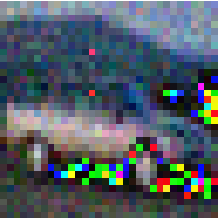
\includegraphics[height = 2.3cm]{images/protecting/Zhang-038.png}}
            \hfill
    \subfloat[Perturb. \cite{merrer_adversarial_2019}\label{fig:trigger-e}]{%
        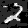
\includegraphics[height = 2.3cm]{images/frontier/merrer-011.png}}
        
    \caption{Examples for the various types of trigger images, intentionally labelled as a different class ((a), (b) as "cat", (c), (d) as "airplane", (e) as "9")}
    \label{fig:blackbox}
\end{figure*}
% -------------------------- %

Zhang et al. \cite{zhang_protecting_2018} propose the first black-box watermarking scheme in 2018 and introduce three types of trigger images: \textit{unrelated} (OOD), \textit{content} (pattern based) and \textit{noise} (based). %, as described above.
Their work forms the basis for many following papers.
%prime candidate for deletion. Can also be moved to an appendix where we gather some peculiar stuff. But I think it clearly fulfills our exclusion criterion.
%For the sake of completeness, we note that Zhang et al.'s work got re-implemented by Deeba et al. \cite{deeba_digital_2020}\footnote{Earlier version \cite{deeba_protecting_2019}} on another dataset. Their evaluation do not reveal any negative aspects of Zhang et al.'s work.

\subsection{Out-of-distribution}
Similar to and shortly after Zhang et al. \cite{zhang_protecting_2018}, Adi et al. \cite{adi_turning_2018} propose to include abstract images as trigger images in the training dataset. Those abstract images are completely unrelated to the main classification task% of the trained model
, thus it is highly unlikely that a model that has not seen this data point (i.e. one not watermarked) will label it as the designated class. %Furthermore, they proposed to combine the embedding with a \textit{commitment scheme} for more security.

% ---- Quan: Watermarking Deep Neural Networks in Image Processing
%TODO: how are the inputs generated? using something specific?
One of the first watermarking schemes for image processing models was proposed by Quan et al. \cite{quan_watermarking_2020}. The main difference to classification is that the output is, like the input, an image and not a label -- thus they are generating input-output pairs which consist of trigger images and verification images. They propose to use OOD images (or random noise) as trigger images and create the verification images by applying a simple image processing method to the trigger images (ideally not the one trained by the model). The idea is the same as in (defensive) backdooring. They generate input-output pairs where each consists of a trigger image and a verification image. The model is then fine-tuned on the union of the training dataset and the trigger set.
%The watermark verification is performed by querying the trigger image and comparing the output image with the verification image.

% ----- Yang: Effectiveness of Distillation Attack and Countermeasure on Neural Network Watermarking --- does not rely on specific choice of trigger images
Yang et al. \cite{yang_effectiveness_2019} empirically show that distillation is an effective watermark removal attack.
%Distillation is a type of compression where the knowledge of the original model (teacher model) is distilled into another smaller model (student model) \cite{hinton_distilling_2015}.
Therefore, they propose a new watermarking scheme, called \textit{ingrain}, that the authors claim to be especially robust against distillation. The main idea is that the watermark information is carried by the predictions of the original training data but the watermark extraction is done by querying trigger images that are drawn from a different distribution than the original images. Comparing to \cite{adi_turning_2018} and \cite{zhang_protecting_2018}, the target model is not trained on the union of the original training dataset and the trigger set, but only on the original dataset, and instead makes use of another model, the \textit{ingrainer model}, which influences the target model by a regulariser term to the loss function. The ingrainer model has the same architecture as the target model and is only trained on the trigger set, in particular, to overfit the trigger set.
%Roughly speaking, the model for the main classification task $\mathcal{F}_{\mathbf{w}}$ is influenced by another model, the ingrainer model $\mathcal{G}_{\mathbf{\theta}}$, which carries the watermark information, has the same architecture as the original model and is trained on the trigger set, in particular to overfit the trigger set.
% The ingrainer model stays fixed in the process of training the original model. The original model is then trained on both the original dataset and the trigger set. The influence of the ingrainer model is attained by adding a regulariser term to the loss function which is controlled by the ingrainer model $\mathcal{G}_{\theta}$.

\subsection{Pattern} \label{sec:black-box:pattern}
% ------ Li: Piracy Resistant Watermarks for DNNs
An improved pattern based technique was proposed by Li et al. \cite{li_piracy_2020}. They show that previous schemes \cite{adi_turning_2018, zhang_protecting_2018} are vulnerable to \textit{ownership piracy} attacks, in which an attacker aims to embed his own watermark into an already watermarked model. They propose a watermarking scheme that is especially robust against such attacks using \textit{dual embedding}: %, combining null embedding and true embedding.
the model is trained to classify (i) data with a pre-defined binary pattern correctly (\textit{null embedding}), and (ii) data with an inverted pattern (binary bits are switched) incorrectly (\textit{true embedding}). 
In more detail, for a pre-defined binary valued pattern $p$ and a very large number $\lambda$, the pattern $p$ is dual embedded into the model $\mathcal{F}_w$ if for all $X \in \mathbb{R}^n$ holds
\begin{align}
     \mathcal{F}_w(\mathrm{apply}(X, p, \lambda)) = \mathcal{F}_w(X) = y, \label{eq:nullembedding} \\ 
     \mathcal{F}_w(\mathrm{apply}(X, \mathrm{inv}(p), \lambda)) = \hat{y} \neq y, \label{eq:trueembedding}
\end{align}
where $\mathrm{apply}(X, p, \lambda)$ applies the pattern $p$ with magnitude $\lambda$ (value $\lambda$ for bit 1 and value $-\lambda$ for bit 0) to the image $X$. \cref{eq:nullembedding} refers to null embedding and \cref{eq:trueembedding} to true embedding.
%In null embedding the model is trained to classify the data with an embedded binary pattern correctly and in true embedding the model is trained in a way that images with an inverted pattern (binary bits are switched) are classified incorrectly.
% We define dual embedding: for a pre-defined binary valued pattern $p$ and a very large number $\lambda$, the pattern $p$ is dual embedded into the DNN model $\mathcal{F}_w$ if for all $X \in \mathbb{R}^n$ holds
% \begin{align}
%     \mathcal{F}_w(\mathrm{apply}(X, p, \lambda)) = \mathcal{F}_w(X) = y, \label{eq:nullembedding} \\ 
%     \mathcal{F}_w(\mathrm{apply}(X, \mathrm{inv}(p), \lambda)) = y_w \neq y, \label{eq:trueembedding}
% \end{align}
% where $\mathrm{apply}(X, p, \lambda)$ applies the pattern $p$ with magnitude $\lambda$ (value $\lambda$ for bit 1 and value $-\lambda$ for bit 0) to the image $X$. \cref{eq:nullembedding} refers to null embedding and \cref{eq:trueembedding} to true embedding. $\mathrm{inv}(p)$ denotes the inverted pattern, which means that the binary values in $p$ are switched. When the inverted pattern is applied, the model is trained to predict any other label $y_w$ than the original label.
They observe that null embedding does not degrade the model's accuracy if the number of pixels in the pattern is sufficiently small.
%and that "once a model is trained and null embedded, an adversary cannot null embed a pirate pattern without largely degrading the model's classification accuracy". 
% This scheme differs from other works because it uses large values $\lambda$ to generate the trigger image and therefore is more robust against backdoor detection like Neural Cleanse \cite{wang_neural_2019}.
Furthermore, they evaluate the robustness against model extraction attacks and conclude that, with enough (at least the same amount of) in-distribution data, the attacker is able to make a copy of the model without the watermark. For out-of-distribution data, the attacker would need 12.75 times more input data to reach similar accuracy.

% ---- Guo: Watermarking Deep Neural Networks for Embedded Systems
Guo et al. \cite{guo_watermarking_2018} propose to embed a pattern into the trigger images that can be clearly associated with the model owner's signature, e.g. a logo. The pattern should be embedded with little visibility so that the original model would still classify the trigger images to their original labels. The signature is used as a key to determine the pattern and then embedded in the image.% with an adjustable magnitude. 
%After embedding the watermark into the model, in other words after training the model with the original training set augmented by the trigger set, the watermarked model will be able to recognise images with the embedded pattern, and label them to a different class than the original one.
%The proposed way to create a unique pattern is the following: the model owner generates the $T$-bit signature by hashing a message and uses it as the key to a pseudorandom random permutation, which will define the location of the $T$ pixels, that will be changed. The 0/1-bits from the signature are transformed to -1/1 values and located on the defined pixels, which all together will form a pattern $p$ that will be added to the image $X$ with an adjustable magnitude $\alpha$.

% ---- Evolutionary trigger set generation --- pattern based
Guo et al. \cite{guo_evolutionary_2019} propose an evolutionary algorithm-based method to generate and position trigger patterns, based on \cite{zhang_protecting_2018} and \cite{guo_watermarking_2018}. %This should lead to a significant reduction in false positive rates of the watermarked model.
Their algorithm is based on Differential Evolution \cite{storn_differential_1997}, %TODO: remove reference if we need reference space
an evolutionary algorithm and a metaheuristic that searches for the optimal solution for an optimisation problem.
%TODO: describe what is the optimisation - position for log embedding? what for noise?
Using this trigger pattern generation they demonstrated an improvement in integrity and robustness.
% Nur für mich, als Info. Bin mir noch nicht sicher, ob ich das erwähne:
% It is worth noting that "Guo et al. found that embedding a new watermark using limited amount of data would degrade the model's performance. Therefore, they ruled out this possibility of attack."

\subsection{Noise}
% ---- Secure NN WM protocol --- noise?
Zhu et al. \cite{zhu_secure_2020} propose a watermarking scheme especially to defend against watermark overwriting (forging attacks). They propose to use one-way hash functions for both generating the trigger image and label.
%trigger image generation. Let $H_X$ be a hash function that takes an image and a key as input and outputs an image and $H_y$ a hash function that takes an image as input and outputs an integer value. $H_X$ is used to generate the trigger images and $H_y$ to generate the corresponding labels.
The framework takes an initial image and creates a hash chain of trigger images, as shown in \cref{fig:zhu}. They show experimentally that their proposed scheme is robust against forging attack even if the attacker knows the trigger set generation algorithm.
%protocol for trigger generation.

\begin{figure}[t]
    \centering
    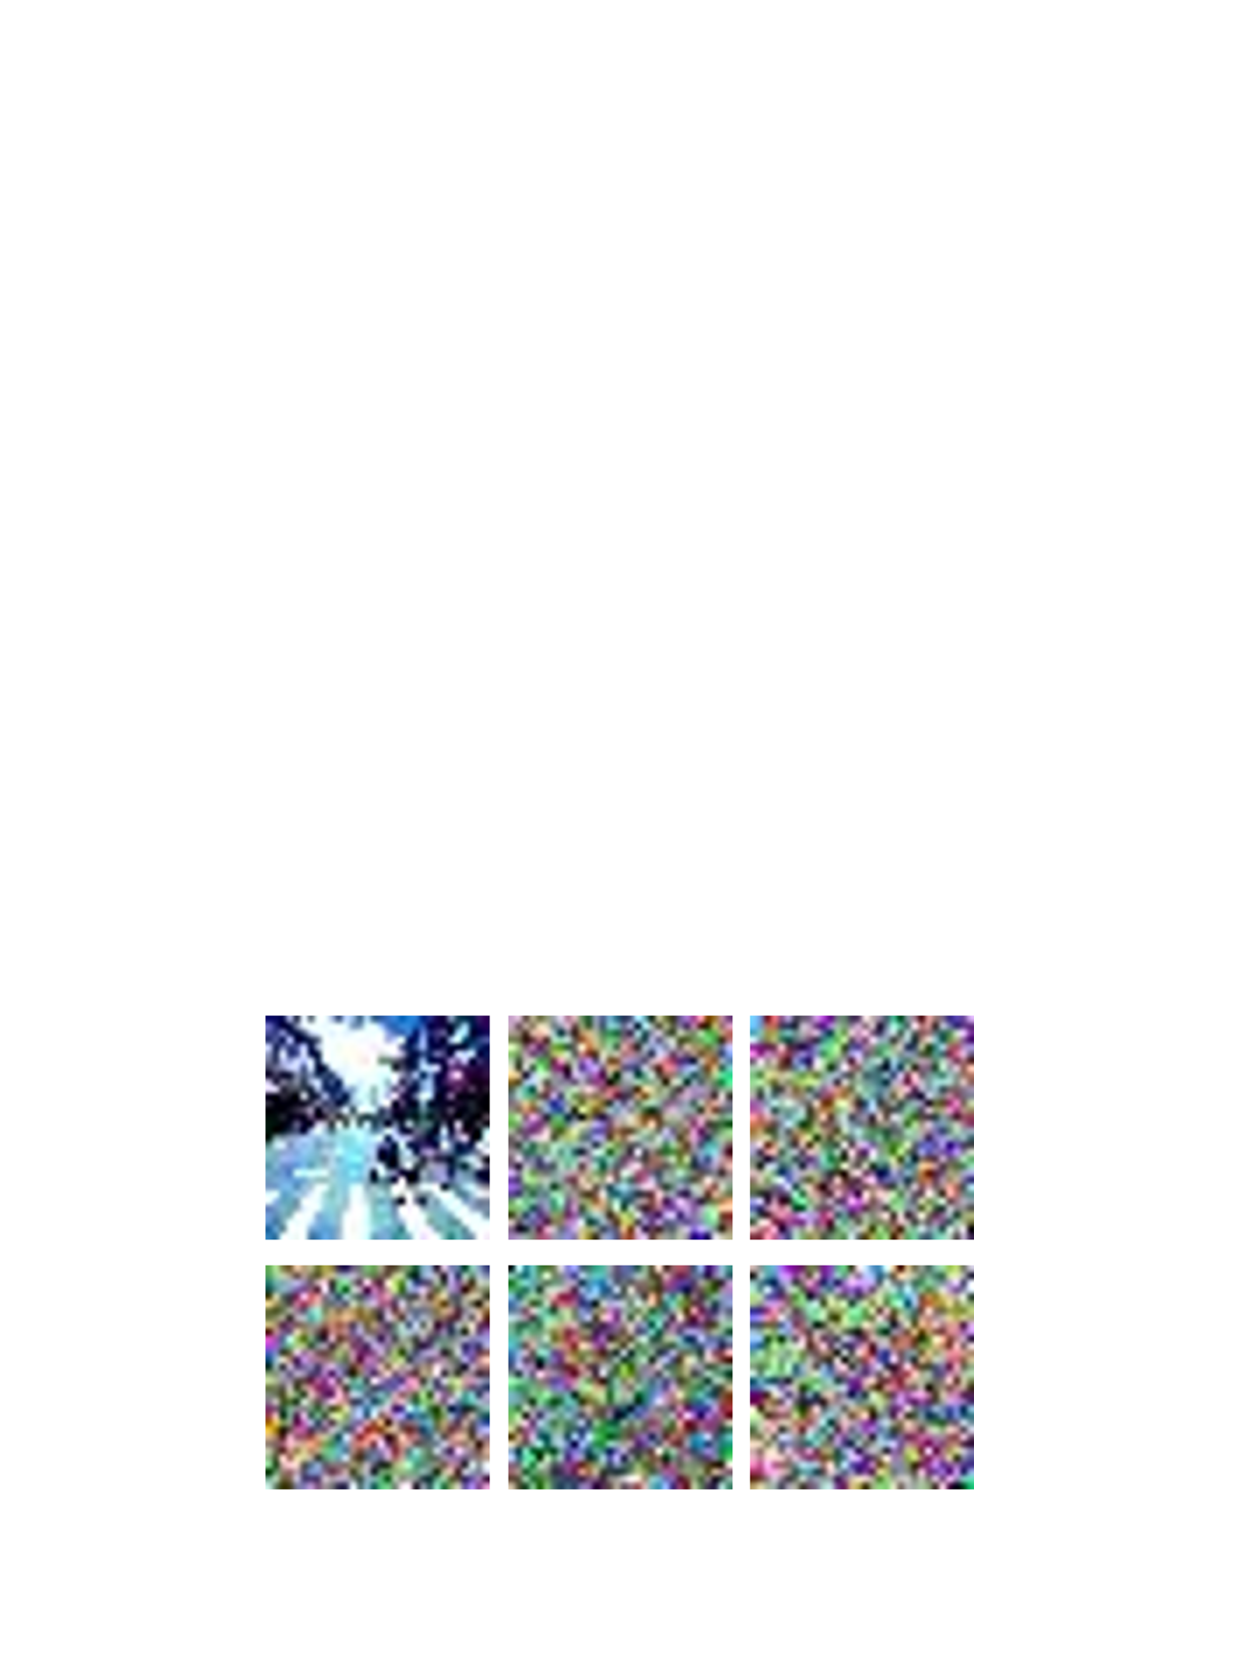
\includegraphics[width = 0.4 \textwidth]{images/Zhu1.pdf}
    \caption{The upper left image is the initial image and the following five are trigger images resulting from a hash chain \cite{zhu_secure_2020}.}
    \label{fig:zhu}
\end{figure}

\subsection{Perturbation}
% ---- adversarial frontier stitching
Another black-box scheme was proposed by Merrer et al. \cite{merrer_adversarial_2019}. The goal is to slightly shift the decision boundary of the model. This is achieved by generating adversarial examples \cite{szegedy_intriguing_2014} for images close to the boundary, and changing the class for those adversaries. % to the neighbouring class.
After fine-tuning the model, the decision boundary is adapted. An illustration of this decision boundary shifting for a two class boundary is given in \cref{fig:merrer}.

\begin{figure}[t]
    \centering
    \hspace*{\fill}
  \subfloat[\label{fig:merrer-a}]{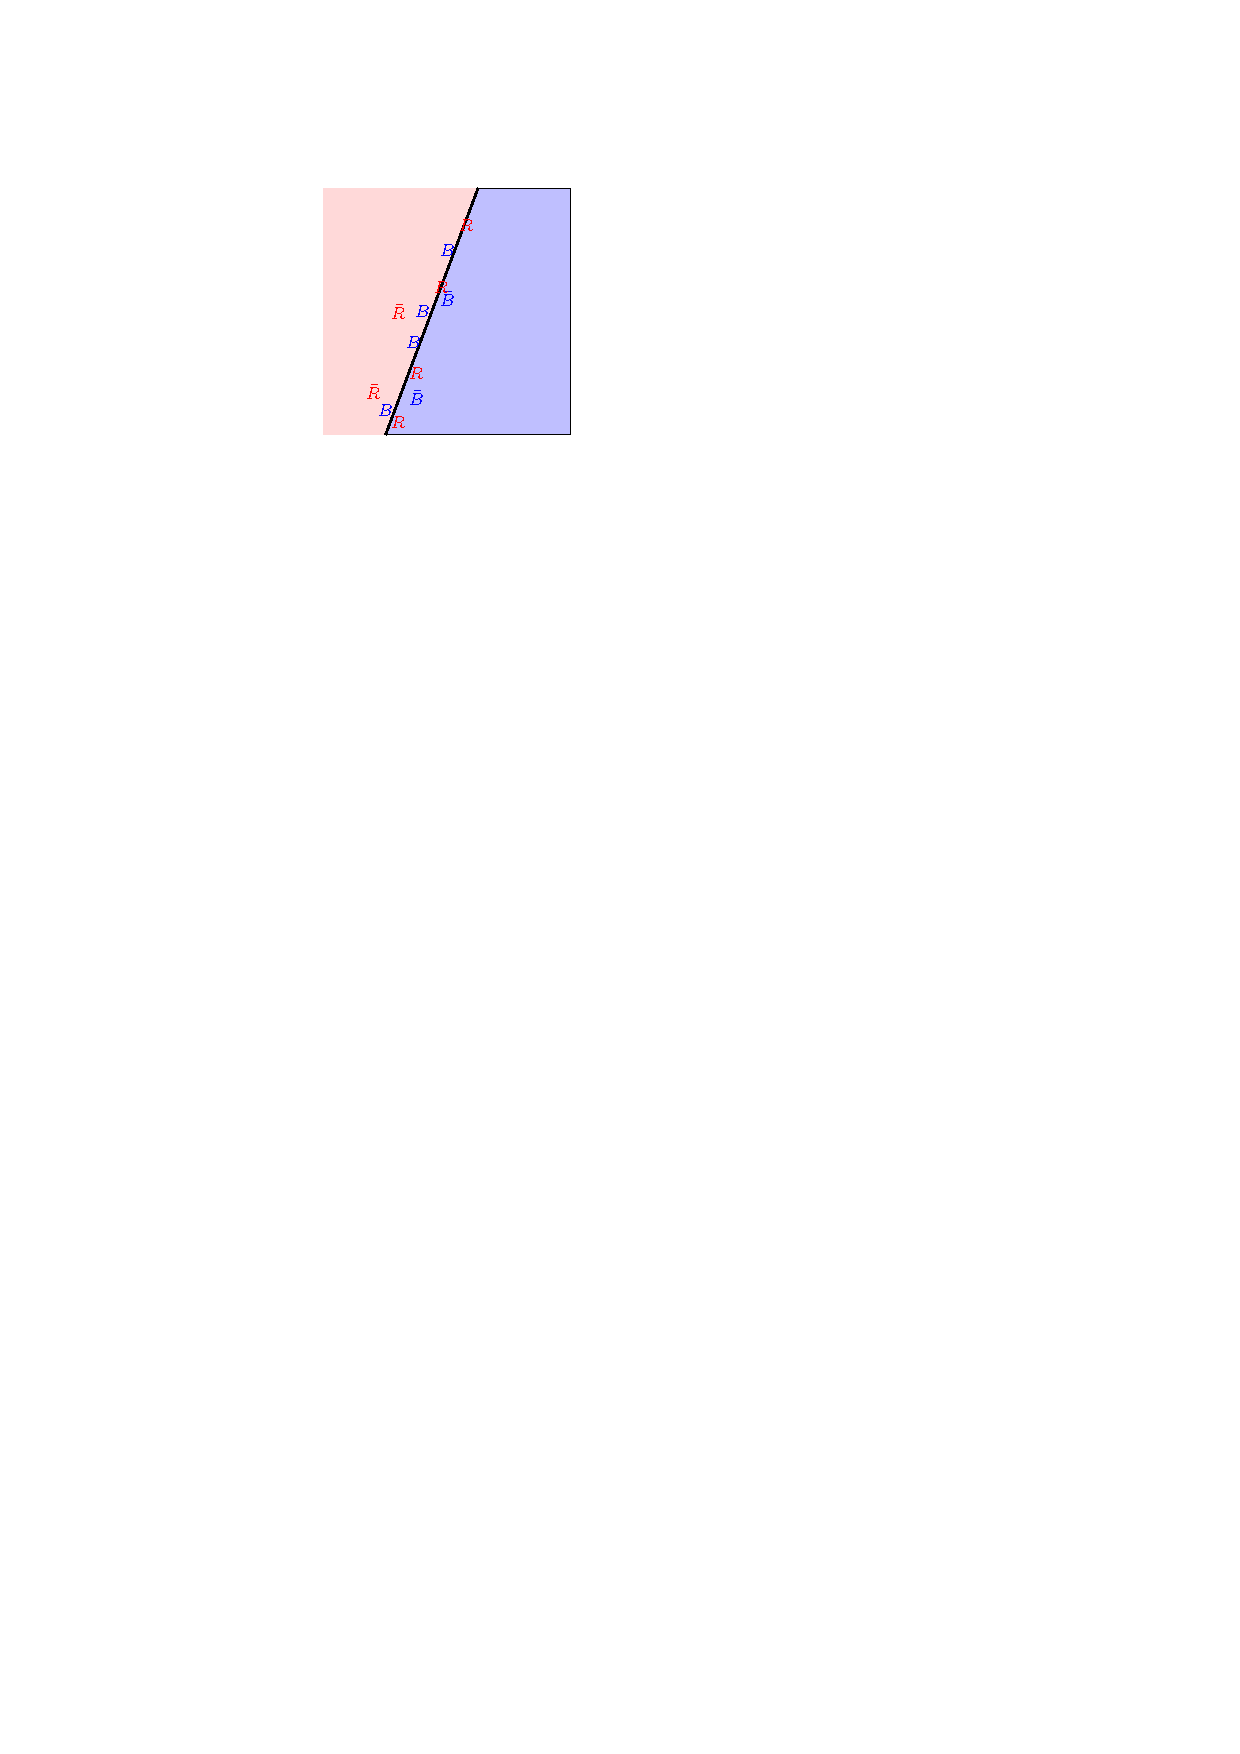
\includegraphics[width = 0.2 \textwidth]{images/frontier/Merrer1.pdf}}
    \quad
  \subfloat[\label{fig:merrer-b}]{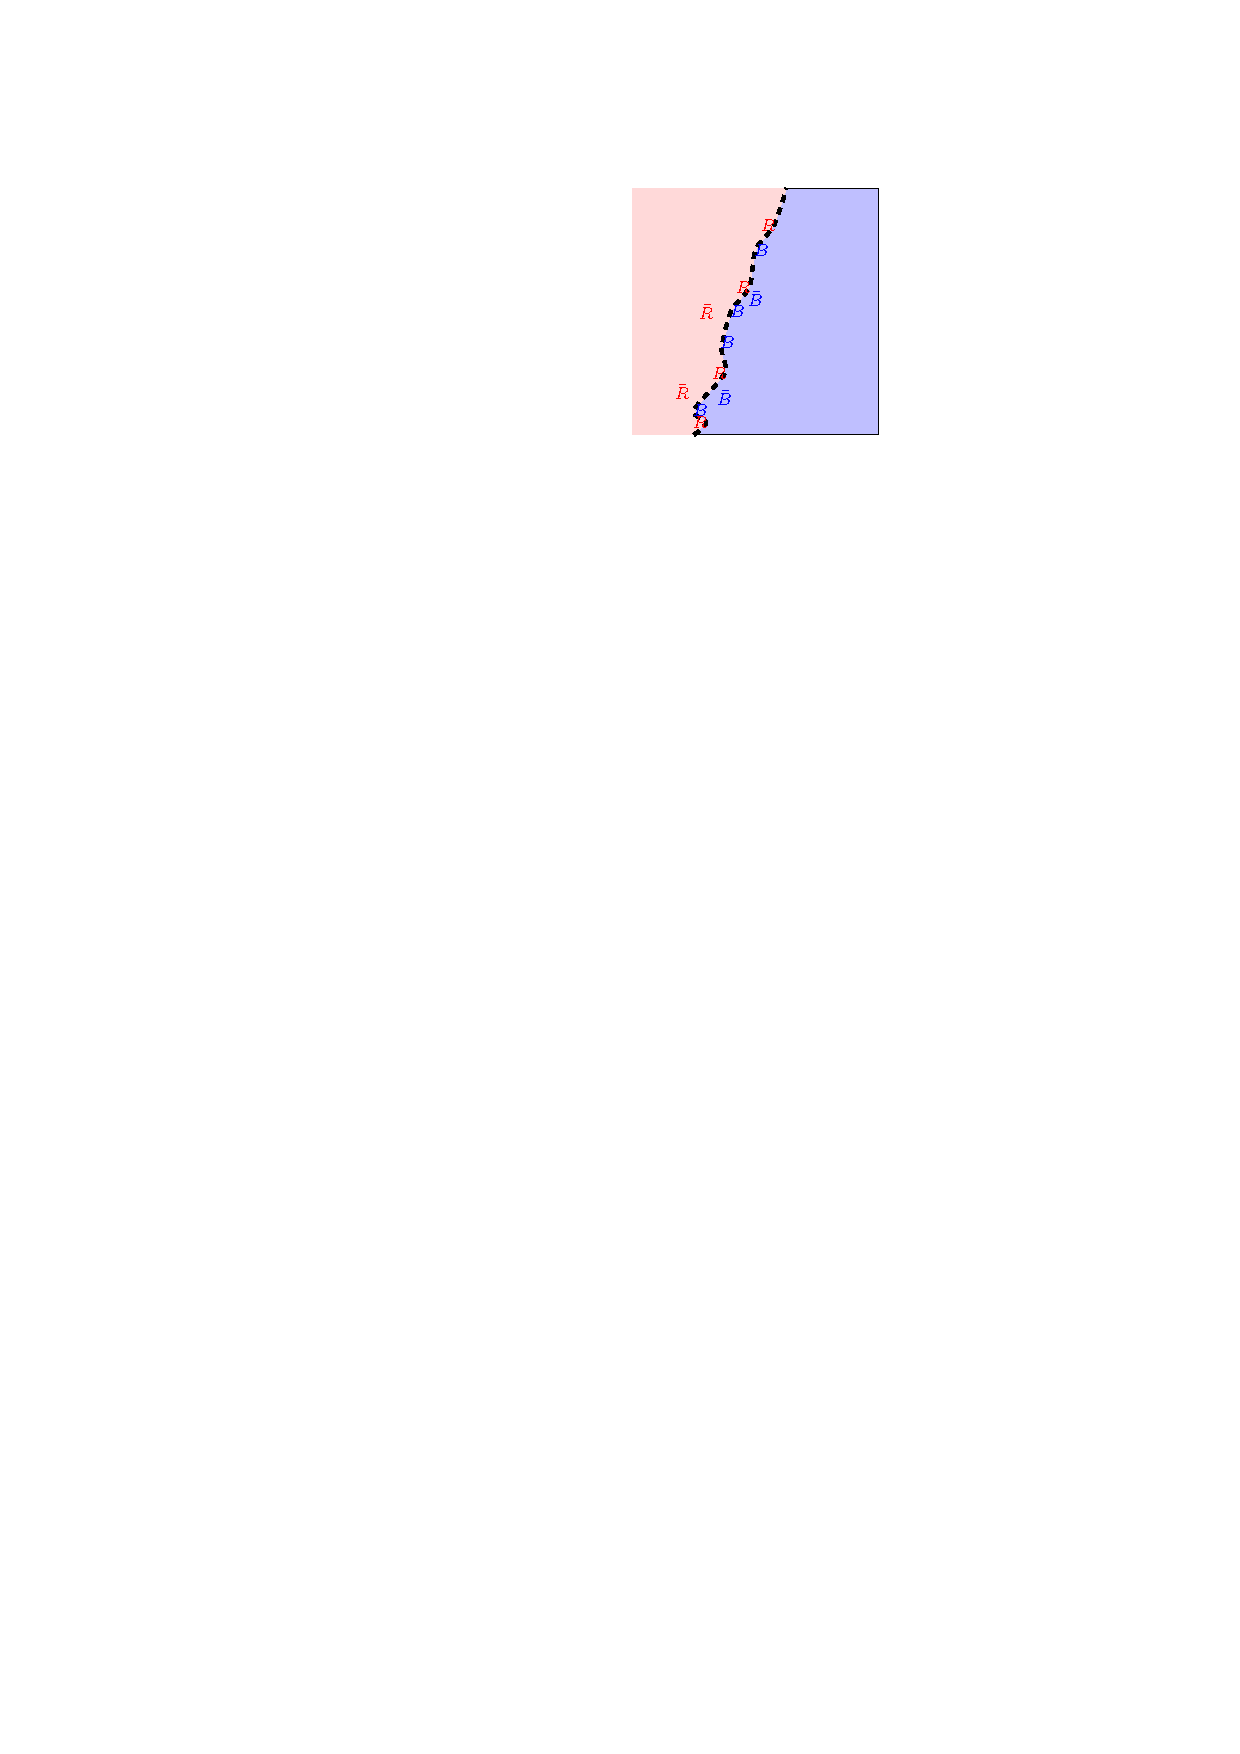
\includegraphics[width = 0.2 \textwidth]{images/frontier/Merrer2.pdf}}
    \hspace*{\fill}
    \caption{(a) The data points are divided into "true adversaries" ($R$ and $B$) and "false adversaries" ($\bar{R}$ and $\bar{B}$). The label for the true adversaries is changed, the label for the false adversaries stays unchanged. (b) After fine-tuning the decision boundary changes. \cite{merrer_adversarial_2019}}
    \label{fig:merrer}
\end{figure}

% ----- GAN-based technique
Li et al. \cite{li_how_2019} especially address evasion attacks. They propose a framework closely related to the idea of GANs. They use three DNNs: encoder, discriminator, and target model. The encoder takes the original image and aims to embed a logo into the image such that the difference is imperceptible. The resulting trigger images are fed into the discriminator together with the original image to evaluate the encoder's success.
%detect if the trigger image was generated by the encoder. 
%The networks are trained iteratively until they reach their optimum.
%Finally, the target model is trained with the original images together with the generated trigger images.
A difference in the original and trigger images is essential for the watermarking scheme, yet the goal is to make the difference as small as possible. This framework especially deals with the trade-off between security and effectiveness. The smaller the difference, the better security against evasion attacks, and the larger, the better the effectiveness of the embedded watermark.

% ---- Chen: BlackMarks - nicht sicher ob ich zu perturbation zuordnen kann
Chen et al. \cite{chen_blackmarks_2019} propose the watermarking framework \textit{BlackMarks}, which %embeds a binary signature into a model and can be verified in the black-box setting.
encodes the signature within the distribution of the output activations. % (before applying softmax). %, and creates targeted adversarial attacks as trigger images.% and labels.
To encode the class predictions, the authors design a scheme that maps the class predictions to binary bits, by clustering the original classes into two categories, represented by bit 0 and bit 1. The trigger images are created in a way that for the bit 0, an adversarial example that would belong to the cluster represented by the bit 1 is created, and is labelled with a uniformly randomly chosen class from the cluster represented by the bit 0. Trigger images for the bit 1 are created vice-versa. The watermark is extracted by querying the trigger images and encoding each class to a binary value, which should result in the owner's binary signature to prove ownership.

\subsection{In-distribution}
Namba et al. \cite{namba_robust_2019} propose an attack, called \textit{query modification}, that investigates the query for trigger images in order to invalidate the watermark (cf. \cref{sec:attacks}). With that in mind, they propose a scheme that is more robust especially against query modification but also model modifications like fine-tuning and model compression (e.g. pruning). The query modification as an attack exploits the fact that trigger images differ from original training images. Therefore, they propose to use trigger images that are selected from the training sample distribution.
%They randomly select a sample of images from the training data and change the label, e.g. from "dog" to "cat". After embedding, the model will classify, for instance, all dog images correctly but only this specific one as "cat".
The trigger images are thus undetectable, however, the model is more likely to overfit to the (on purpose) wrongly labelled triggers, and thus more susceptible to removal attacks via e.g. pruning. They want to counter pruning by ensuring that the predictions do not depend on a large number of small model parameters that would likely be pruned. Thus, the model is first trained as usual with the original training set. Then, the watermark is embedded by exponentially weighting the parameters and training the model on the union of the training dataset and the trigger set, which enforces the predictions to depend on a small number of large parameters instead.
In exponential weighting the model parameters $\mathbf{w}^l$ are changed in every layer $l$ by
\begin{align} \label{eq:exponential-weighting}
     \mathbf{w}_{\mathrm{exp},i}^l = \frac{\lambda \mathrm{exp}\, |\mathbf{w}_i^l|}{\mathrm{max}_i \, \lambda \mathrm{exp} \, |\mathbf{w}_i^l|}\mathbf{w}_i^l,
\end{align} %in original paper: theta statt w und T statt lambda
where $\mathbf{w}_i^l$ denotes the $i$-th component of the parameter vector $\mathbf{w}^l$ in layer $l$ and $\lambda$ is an adjustable parameter for the intensity of the weighting.

\subsection{Trigger labelling}
% ----- Zhong: Protecting IP of Deep Neural Networks with Watermarking: A New Label Helps --- does not rely on specific choice of pattern
Zhong et al. \cite{lauw_protecting_2020} propose to label the trigger images with a completely new label, rather than assigning one from the existing labels, so that the watermark embedding has only little impact on the original classification boundaries.
Any pattern based trigger image can be used in this context. They compare their work to \cite{zhang_protecting_2018} in their experimental evaluation and show that the proposed scheme achieves a zero false-positive rate, i.e. excellent integrity, and is more robust against fine-tuning and model compression.

Zhang et al. \cite{zhang_deeptrigger_2020} observe that frequently, trigger images are created in a systematic way, and it is thus easier for an attacker to re-create them.
Therefore, they propose to include unpredictability in the labels assigned to the trigger images. They use a chaos-based labelling scheme for trigger images that ensures that an attacker cannot produce a valid trigger set, even if he knows the trigger pattern.

% ----- Xu: Identity Bracelets --- does not rely on specific choice of trigger images
Xu et al. \cite{xu_identity_2020}\footnote{Previous pre-print version in \cite{xu_novel_2019}} propose, similar to \textit{BlackMarks} \cite{chen_blackmarks_2019}, a watermarking scheme that carries the watermark information within the output activations. The trigger pairs consist of a trigger image and a serial number (SN) which is constructed individually by the owner's rules. The SN is composed by using the probabilities in the last layer.
%For instance, for the MNIST dataset, which has 10 different classes, the SN could be a 10 digit number but also a 20 digit number by adding zeros to the classical 10 dimensional one-hot encoding. In particular, if the generated SN is "558831271817-2355-7965", the digits must be reduced by two orders of magnitude and added 0.001. The resulting probabilities that should be predicted by the given trigger images are [0.051, 0.051, 0.081, 0.081, 0.031, 0.011, 0.021, 0.071, 0.011, 0.081, 0.011, 0.071, 0.021, 0.031, 0.051, 0.051, 0.071, 0.091, 0.061, 0.051].
It is worth noting that any rule for generating it is feasible. For instance, for three classes the SN could be "235" following the rule to reduce the digits by one order, resulting in [0.2, 0.3, 0.5], but also any other, more complex rule can be used. The proposed scheme does not rely on the specific choice of trigger images since it focuses on the output activations. 

\subsection{Countering Model Extraction} \label{sec:wm:countering_extraction}
% --- Jia: EWE
Only a few schemes address the second threat model case in \cref{sec:threatmodel}, i.e. robustness against model extraction attacks. %, we have to consider other watermarking frameworks than the ones introduced before.
Jia et al. \cite{jia_entangled_2020} are the first to propose a scheme, called \textit{entangled watermark embedding} (EWE). %, which they claim and evaluate to be robust against tested model extraction techniques.
%They observe that watermarks are usually outliers in the distribution of the training data and that watermarked models can be separated into two sub-models, one for the main task and the other one for watermarking. The latter one usually does not survive model extraction.
The main idea is to create a watermarked model that is not specialised into "sub-models", where one part of the model is capable of the main classification task, and the other for watermark detection (which normally is lost during the model extraction attack). This is achieved by a regulariser term ensuring that the trigger images lead to similar activation patterns as the original images. Thus, both trigger images and original images cause a similar behaviour of the model, thereby increasing the robustness against model extraction.  
% They make use of the soft nearest neighbour loss (SNNL) \cite{kornblith_similarity_2019, salakhutdinov_learning_2007}. %TODO: if space is needed in references, remove one of those two
%"which measures the distance between points from different groups relative to the average distance for points within the same group."
%Data points are forming clusters when the SNNL is minimised and they are entangled when the SNNL is maximised.
%In EWE, the trigger images generation works as follows: two similar classes are chosen. If the images from the classes are similar, it will be easier to entangle them. 
%The trigger pattern is chosen and the location for the pattern is determined where the gradient of the SNNL is largest. During embedding, the negative SNNL is used as a regulariser term in the fine-tuning process. In this way, the watermarks and original data points are entangled and more robust against extraction attacks.
% TODO: could mention that they also test their scheme for audio classification

% ---- Szyller: DAWN
%Another defence against model extraction was proposed by 
Szyller et al. \cite{szyller_dawn_2020} propose the framework \textit{Dynamic Adversarial Watermarking of Neural Networks} (DAWN), which is not embedding a signature into the target model itself but dynamically returning wrong classes from the API service for a fraction of queries to mark an adversary model created via a model extraction attack.
It is worth noting that the scheme is not able to differentiate between an attacker and a benign client -- all clients obtain a fraction of wrong predictions. %Whether a specific response should be watermarked, and which wrong class to use for the watermark, is based on a hash function.
%keyed cryptographic hash function as a source for randomness.
It is ensured that the same query always returns the same output (correct or modified). Whenever a wrong prediction is returned, the input-output pair is saved so that in need of a watermark verification, they can be used for triggering the stolen model. This approach thus realises \circled{4} in \cref{fig:watermarking-ml-process}.

% ---- Zhang: Model Watermarking for Image Processing Networks
Zhang et al. \cite{zhang_model_2020} and Wu et al. \cite{wu_watermarking_2020} propose, independently of each other, a similar approach to \cite{szyller_dawn_2020}, as they are hiding an invisible watermark in the outputs of the image processing model, but for \textit{all} outputs. When an attacker trains a new (surrogate) model on the input-output pairs of the original model, the watermark will be learned too and can be verified with black-box access (cf. \circled{4} in \cref{fig:watermarking-ml-process}). The major difference to \cite{szyller_dawn_2020} is that in the case of an image processing model, the output is another image, and thus there is more data to embed the watermark in. Both papers are not explicitly addressing model extraction attacks, but we believe they are a suitable defence.
%Wu et al. train a target network, which learns to embed the watermark, and a watermark extraction network, which learns to extract the watermark, together by optimising a combined loss function.

% % ------ Wu: Watermarking Neural Networks with Watermarked Images
% is similar to Zhang above. Unified those two.
% Wu et al. \cite{wu_watermarking_2020} proposed a black-box model watermarking framework for image processing models that watermarks every ouput of the model, like \cite{zhang_model_2020}. They train a target network, which learns to embed the watermark, and a watermark extraction network, which learns to extract the watermark, together by optimising a combined loss function.

\subsection{Watermarking for specific ML settings}
% % ---- Sakazawa: Visual Decoding of Hidden Watermark in Trained Deep Neural Network
% In contrast to other work, which mainly focuses on watermark embedding, Sakazawa et al. \cite{sakazawa_visual_2019} focuses on the watermark extraction. They propose a "cumulative and visual decoding" of watermarks in deep neural networks and experimentally show that their proposed method can successfully decode simple watermarks from trigger images.
% % nicht in requirements tabelle weil keine embedding methode

%---> paper sieht sehr mies aus.

% ------ Atli: WAFFLE: Watermarking in Federated Learning
% "framework"
Existing watermarking schemes are not suitable for Federated Learning (FL), as pointed out by Atli et al. \cite{atli_waffle_2020}. Embedding a watermark in such a setting is different, because the model owner has no access to training data, and the training is performed in parallel by several clients.
%Therefore, the model owner cannot embed the watermark on the training data and neither the clients because one of them could be malicious.
Atli et al. %developed a black-box watermarking scheme for client-server FL via backdooring. They 
propose to include an independent and trusted party between the model owner and the clients. The independent party has the ability to embed a black-box watermark based on backdoors into the model at every aggregation step.
%Could be deleted, not essential. But maybe moved to noise pattern section?
Furthermore, they propose a watermarking pattern that is a specific noise pattern.
% Ist nicht in den requirements tables enthalten. Weil nicht vergleichbar mit den anderen. Listet ähnliche aber dennoch sehr spezifische requirements auf.

% ------ Skripniuk: Black-Box Watermarking for Generative Adversarial Networks
Skripniuk et al. \cite{skripniuk_black-box_2020} propose the first, and until now only, watermarking scheme specially crafted for GANs. The existing watermarking schemes are limited to DNNs that map from images to classes, and thus could not be transferred to GANs. The authors watermark the input images and then transfer the watermarked images to the GAN model. First, the image steganography system has to be trained, which consists of an encoder and decoder,
%The encoder takes an image and an watermark and produces a watermarked image, whereas the decoder takes the watermarked image and outputs the embedded watermark.
and subsequently, \textit{all} the training data together with a secret watermark is fed to the encoder resulting in watermarked data. The watermarked data is then used to train the GAN model. For verification, the model owner only needs an output image of the GAN, and applies the decoder on it to compare the result with the secret watermark. Thus, the proposed scheme needs only black-box access for verification.

% ------ Lim: Protect, Show, Attend and Tell: Empower Image Captioning Model with Ownership Protection
Lim et al. \cite{lim_protect_2020} are the first to propose watermarking for a recurrent neural network (RNN). Specifically, they consider an image captioning model, implemented as a simplified variant of the \textit{Show, Attend and Tell} model \cite{xu_show_2015}, where the output of the model is a sequence (the caption). The proposed framework is similar to \cite{fan_rethinking_2019}, but does not embed the verification information (the owner's key) into the model weights, but into the signs of the hidden states of the RNN.
During model inference time, the key is required as input to the model by an element-wise combination with the input data.
Without the correct key provided, the effectiveness of the model drops significantly.

\section{Fingerprinting of ML Models} \label{sec:fingerprinting}

Imagine a software company is selling their ML model to different customers, but the model got illegally redistributed by one of them. The company would like to gather evidence on the leak and therefore could embed fingerprints in the ML model before selling the product, in order to trace back the user when needed. We can think of fingerprinting as an extension of watermarking on a user level.
%
At the time of performing this survey, fingerprinting for ML models was not extensively discussed, with only three papers %on this topic were 
published.

Note that there is another notion of fingerprinting. In cyber security, a (unique) identifier for an object (either hardware, software, or a combination thereof) is generally referred to as a fingerprint, e.g. such as in browser fingerprinting~\cite{eckersley_how_2010} or device fingerprinting~\cite{kohno_remote_2005}. The application scenario for employing these techniques is often in tracking devices (resp. their users). Because this context differs from what we considered so far, we call this form \textit{Fingerprinting as unique identification}.

\subsection{Fingerprinting as User-specific Watermark}
\label{sec:fingerprinting:user-specific-wm}
%The owner wants to distribute a model to multiple users, each having an individual fingerprint embedded in the model, to verify the malicious user in case of ownership infringement.

% regulariser based
Chen et al. \cite{chen_deepmarks_2019} propose a white-box fingerprinting framework, \textit{DeepMarks}, that is able to embed unique fingerprints. The verification process not only detects the attacker, but detects also if multiple, and if so which, users collaborated in order to create an unmarked model. The embedding process works similar to the one in \cite{rouhani_deepsigns_2019}. They propose to assign a unique binary vector (fingerprint) to each user and embed the fingerprint information in the PDF of the weights before distributing the models to the users.

Although \textit{DeepMarks} is the only paper considering especially fingerprinting, we believe that a couple of the above introduced watermarking schemes can be extended to fingerprinting. To name a few, \cite{uchida_embedding_2017} embeds a unique signature into the weights of the DNN, \cite{li_how_2019} embeds a unique logo into the trigger images and \cite{guo_watermarking_2018} generates unique trigger images based on a signature. All of them could embed user-specific watermarks. Moreover, \cite{xu_identity_2020} relies on serial numbers that can be created in indefinitely many ways, assigning each to a user.

\subsection{Fingerprinting as Unique Model Identifier}
%However, a unique identification of a ML model is not secure enough for our threat model. For example, 
Cao et al. \cite{cao_ipguard_2020} propose a framework to obtain a unique identifier of DNNs. %by "fingerprinting" the classification boundary of DNNs.
Based on the idea that two different models have different classification boundaries, they propose to "fingerprint" the classification boundary of the model. If the model was changed in the slightest way, the classification boundary would slightly shift too. This scheme, however, does not fit our threat model, as we want to recognise the original model even after (especially minute) model modifications. We, therefore, require a fingerprinting framework to be more robust to model modifications.

% also fan_rethinking_2019 mentions a "signature" of signs in some layers as fingerprint / signature string

% perturbation
% man könnte diesen Absatz natürlich auch zu perturbation based geben. Der Unterschied ist, zB zu Merrer (der extra trigger images nahe zur classification boundary generiert und dann damit fine-tuned um die classification boundary etwas zu shiften), dass sie die adversarial images finden, aber dann in das model einbetten.
Zhao et al. \cite{zhao_afa_2019} and Lukas et al. \cite{lukas_deep_2020} modify this idea of fingerprinting as unique identification. Both propose a scheme in which the adversary model, created by applying modifications to the target model, has the same fingerprint as the target model. They both introduce a novel algorithm for creating transferable adversarial examples \cite{liu_delving_2017}. %These adversarial examples are slightly different from the original image but different enough to fool the model to classify the image incorrectly.

Note that in \cref{sec:blackbox} we describe how black-box watermarking methods use perturbation based trigger images (adversarial examples), which are used during training so that the models learn how to (purposefully) misclassify them.
In the context of fingerprinting as a unique model identifier, the authors want to create an adversarial example from an already trained ML model. The key aspect is that the generated images are not only adversarial examples for the target model, but also for the adversary model, i.e. they are transferable to the adversary model. This %, in contrary to Cao et al.'s work \cite{cao_ipguard_2020}, 
fits our first threat model case in \cref{sec:threatmodel}.

\section{Attacks on Watermarking Methods}
\label{sec:attacks}

If the attacker knows or suspects that a model is protected, he could try to change the model in order to remove or overwrite the protection. 
Regarding watermarking, most authors claim that their techniques are robust against various model modifications like \textit{fine-tuning}: re-training the model with new data and \textit{parameter pruning}: setting small parameter values to zero, which is a model compression technique \cite{han_deep_2016,zhu_prune_2017}. %molchanov_pruning_2017, li_pruning_2017,
But further attacks were proposed that are aiming to remove, overwrite, detect or invalidate state-of-the-art watermarking schemes, which we will analyse. % We dedicate this section to those works. 
We want to point out that most of the techniques, except of \textit{EWE} \cite{jia_entangled_2020} and \textit{DAWN} \cite{szyller_dawn_2020}, are not robust against model extraction (model stealing) attacks \cite{tramer_stealing_2016}, as pointed out by Mosafi et al. \cite{mosafi_stealing_2019}.

%cell color: \cellcolor[HTML]{ECECEC}

%\begin{table*}[t]
\begin{sidewaystable}
\caption{Which attack defeats which watermarking technique based on the evaluation of the papers. A $\sim$ denotes that the authors claim that their attack can be extended easily to defeat this watermarking technique but did not provide an evaluation for that.} 

\centering
\resizebox{\textwidth}{!}{\begin{tabular}{lll|l|l|l|l|l|l|}
\cline{4-9}
                                                              &                                                            &              &  \multicolumn{6}{l|}{Watermarking techniques}                                                                     \\ \cline{4-9} 
                                                              &                                                            &              & OOD & pattern      & noise       & perturbation & in-distribution & regulariser   based          \\ \hline
 \multicolumn{1}{|l|}{\multirow{12}{*}{\rotatebox[origin=c]{90}{Attacks on watermarks}}} & \multicolumn{1}{l|}{\multirow{2}{*}{invalidation}}         & Hitaj et al. \cite{hitaj_evasion_2019}        & \cite{adi_turning_2018},   \cite{zhang_protecting_2018}$\sim$      &              &             & \cite{merrer_adversarial_2019}$\sim$     &                 &                              \\ \cline{3-9} 
\multicolumn{1}{|l|}{}                                        & \multicolumn{1}{l|}{}                                      & Namba et al. \cite{namba_robust_2019}        & \cite{zhang_protecting_2018}               & \cite{zhang_protecting_2018}        & \cite{zhang_protecting_2018}       & \cite{merrer_adversarial_2019}       &                 & \cite{rouhani_deepsigns_2019}                      \\ \cline{2-9} 
\multicolumn{1}{|l|}{}                                        & \multicolumn{1}{l|}{overwriting}                           & Li et al. \cite{li_piracy_2020}           & \cite{adi_turning_2018}, \cite{zhang_protecting_2018}                 & \cite{zhang_protecting_2018}        & \cite{zhang_protecting_2018}        &              &                 &                              \\ \cline{2-9} 
\multicolumn{1}{|l|}{}                                        & \multicolumn{1}{l|}{detection}                                      & Wang et al. \cite{wang_robust_2020}  &                     &              &             &              &                 & \cite{uchida_embedding_2017},   \cite{rouhani_deepsigns_2019}            \\ \cline{2-9} 
\multicolumn{1}{|l|}{}                                        & \multicolumn{1}{l|}{\multirow{3}{*}{detection,   removal}} & Wang et al. \cite{wang_attacks_2019} &                     &              &             &              &                 & \cite{uchida_embedding_2017}                       \\ \cline{3-9} 
\multicolumn{1}{|l|}{}                                        & \multicolumn{1}{l|}{}                                      & Shafieinejad et al. \cite{shafieinejad_robustness_2019} & \cite{adi_turning_2018},   \cite{zhang_protecting_2018}        & \cite{guo_watermarking_2018},   \cite{zhang_protecting_2018} & \cite{zhang_protecting_2018} &              &                 &                              \\ \cline{2-9} 
\multicolumn{1}{|l|}{}                                        & \multicolumn{1}{l|}{\multirow{5}{*}{removal}}              & Liu et al. \cite{liu_removing_2020}          & \cite{adi_turning_2018},   \cite{zhang_protecting_2018}        & \cite{guo_watermarking_2018},   \cite{zhang_protecting_2018} & \cite{zhang_protecting_2018}       &              &                 &                              \\ \cline{3-9} 
\multicolumn{1}{|l|}{}                                        & \multicolumn{1}{l|}{}                                      & Aiken et al. \cite{aiken_neural_2020}        & \cite{adi_turning_2018},   \cite{zhang_protecting_2018}        & \cite{zhang_protecting_2018}        & \cite{zhang_protecting_2018}       &              &                 &                              \\ \cline{3-9} 
\multicolumn{1}{|l|}{}                                        & \multicolumn{1}{l|}{}                                      & Guo et al. \cite{guo_hidden_2020}          & \cite{adi_turning_2018}                 & \cite{zhang_protecting_2018}        &             & \cite{merrer_adversarial_2019}       &                 &                              \\ \cline{3-9} 
\multicolumn{1}{|l|}{}                                        & \multicolumn{1}{l|}{}                                      & Chen et al. \cite{chen_refit_2020}        & \cite{adi_turning_2018},   \cite{zhang_protecting_2018}        & \cite{zhang_protecting_2018}        &             & \cite{merrer_adversarial_2019}       & \cite{namba_robust_2019}           &                              \\ \cline{3-9} 
\multicolumn{1}{|l|}{}                                        & \multicolumn{1}{l|}{}                                      & Yang et al. \cite{yang_effectiveness_2019}         &                     &              &             &              &                 & \cite{uchida_embedding_2017},   \cite{rouhani_deepsigns_2019}, \cite{chen_deepmarks_2019} \\ \hline
\end{tabular}
}
\label{tab:attacks}
\end{sidewaystable}
%\end{table*}


% \cite{hitaj_evasion_2019}
% \cite{namba_robust_2019}
% \cite{li_piracy_2020}
% \cite{sakazawa_visual_2019}
% \cite{wang_attacks_2019}
% \cite{wang_robust_2020}
% \cite{shafieinejad_robustness_2019}
% \cite{liu_removing_2020}
% \cite{aiken_neural_2020}
% \cite{guo_hidden_2020}
% \cite{chen_refit_2020}
% \cite{yang_effectiveness_2019}

% \cite{adi_turning_2018}
% \cite{zhang_protecting_2018}
% \cite{merrer_adversarial_2019}
% \cite{guo_watermarking_2018}
% \cite{namba_robust_2019}
% \cite{rouhani_deepsigns_2019}
% \cite{uchida_embedding_2017}
% \cite{chen_deepmarks_2019} 
In \cref{tab:attacks}, we summarise the attacks on watermarking schemes.
%, which are going to be discussed in the section.
Each line corresponds to an attack and each column to a (type of) watermarking scheme. The table shows which attack defeats which kind of watermarking. We list only schemes that were proven to be successfully defeated -- missing schemes in the table do not imply strong robustness. We can see that an attack usually addresses either white-box or black-box watermarking schemes. The four trigger image types OOD, pattern, noise and perturbation based seem to be defeated in a similar way. In-distribution watermarks are more difficult to detect or remove, probably because of the fact that they do not differ from the original training data distribution.
%We are going to present the works divided into four types of attacks, which we introduced in \cref{sec:attack-model}: watermark overwriting, detection, removal, and invalidation.
 
\subsection{Watermark Overwriting}
Li et al. \cite{li_piracy_2020} show %, as a motivation for a novel watermarking scheme, 
that previous schemes \cite{adi_turning_2018, zhang_protecting_2018} are vulnerable to watermark overwriting (ownership piracy attack).
%In particular, they show it for \cite{adi_turning_2018} and \cite{zhang_protecting_2018}, pointing out that Wang et al. \cite{wang_attacks_2019} cover already regulariser-based schemes.
They %re-implemented the schemes from the original papers for 
apply the schemes to
four image classification tasks, %: digit recognition (MNIST), face recognition (YouTube Face), traffic sign recognition (GTSRB), and object recognition (CIFAR-10) 
and assume that an attacker would have access to around 10\% of the %5,000
original training images. Experimentally, the authors conclude that an attacker could successfully embed the pirate watermark by training the model with training data that is adapted to the pirate watermark.
  
\subsection{Watermark Detection}
Most black-box watermarking methods are based on backdoors. Therefore, backdoor detection algorithms like Neural Cleanse \cite{wang_neural_2019} and Fine-Pruning \cite{liu_fine-pruning_2018} could be a potential threat to these methods. Wang et al. \cite{wang_robust_2020} show that regulariser based watermarking schemes are vulnerable to watermark detection by the use of a property inference attack \cite{ganju_property_2018}.
Knowing the embedding algorithm, they train a set of shadow models (i.e. models with similar architecture and similar data), some of which will be watermarked, and some not.
From these models, they extract weights as representative features, and subsequently, train a model on these features to distinguish between watermarked and not-watermarked models.

\subsection{Watermark Removal}

Some of the attacks exploit the fact that a watermarked model actually learns two tasks: the main classification task and the watermarking task. This fact can be also observed in the increase of the model parameters' variance during watermark embedding \cite{wang_attacks_2019}.

% ---- Wang: Attacks on Digital Watermarks for Deep Neural Networks - detection and removal -- the variance of the distribution of model parameters
Wang et al. \cite{wang_attacks_2019} are one of the first to reveal serious vulnerabilities in watermarking schemes, in particular watermark detection and removal. They observe that in regulariser based watermarking methods like \cite{uchida_embedding_2017}, the variance of the distribution of model parameters, they call this \textit{weights variance} or \textit{weights standard deviation}, increases during watermark embedding.
%Their detection algorithm measured the variance of model parameters distribution, which they call \textit{weights variance}.
The watermark is removed by embedding one or several additional watermarks into the model, following the embedding scheme in \cite{uchida_embedding_2017}. Since every additional watermark might increase the weights variance, they propose to lower the weights variance by adding a $L_2$ regulariser. Following this procedure, the authors show that the old watermark cannot be extracted, thus the model owner cannot claim ownership anymore. It shall be noted that although additional watermarks are placed into the watermarked model, the main objective is to "neutralise" the old watermark rather than to use the new watermarks to claim ownership.

%In this way, the old watermark can be removed but also the attacker's own watermark can be placed.

% ----- Shafieinejad: On the Robustness of the Backdoor-based Watermarking in Deep Neural Networks -----
Shafieinejad et al. \cite{shafieinejad_robustness_2019} analyse the robustness of backdoor based watermarking schemes. In particular, they propose a model extraction (stealing) attack that trains a substitute model (cf. e.g. \cite{papernot_practical_2017}).
This is performed by querying the original model with a public dataset from the same domain and using the resulting label to train their own model. As the public dataset contains none of the trigger images, the watermark is "lost" in the process.
%steals the functionality of the target model and removes the embedded watermark without having any access to the model's parameters. %Similar to other attacks above, it exploits the fact that the watermarked model actually learns two tasks: the main classification task and the watermarking task, so that trigger images are seen as outliers for the main classification.
%TODO: they also adapt this to a white-box attack
Furthermore, similar to Wang et al. \cite{wang_robust_2020}, they propose to use property inference for watermark detection.
% TODO: haben die auch ein watermarking scheme? ein anderes paper behauptet das -> hätt ich jetzt nicht gefunden...

% ----- Liu: Removing Backdoor-based WM in Neural Networks with Limited Data -----
Liu et al. \cite{liu_removing_2020} propose \textit{WILD}, a framework against backdoor-based watermark techniques based on fine-tuning.
They argue that it is hard for adversaries to collect a large amount of unlabelled data within the same domain as the original training data, as required by \cite{shafieinejad_robustness_2019}, and that using non-domain data impacts the effectiveness of the substitute model.
Their special contribution is that only a small portion of training data is needed. They utilise Random Erasing \cite{zhong_random_2020}, i.e. removing random segments from the input images, to augment the data. %(quote: "to fine-tune the watermarked model robust against occlusion.")
This augmented data alone is, however, not enough to remove a watermark via fine-tuning, because of the high diversity of potential watermarks. They note that backdoor patterns are mostly learned by the high-level feature spaces produced by the convolutional layers, and not by the fully connected layers.
%, especially when only considering the fully-connected layers.
%Therefore, they proposed to consider a high-level feature space and hope
%They further consider fine-tuning once again by considering a high-level feature space. "The intuition behind is that the injected watermarks in neural networks form strongly correlated paths from the input layer to the output layer of the model. We can mitigate the impact of watermarks by weakening the effectiveness of these paths to make the benign object back in control. A good start point that sees all these special kernels is in the high-level feature space just after the final convolutional layer."
%that similarity between data with watermark pattern and clean data implies similarity in the distribution of high-level features of these data points. They %formulated an optimisation problem to minimise the distribution distance between them, and
%\begin{align*}
%\mathrm{minimize}\quad  &d(\mathcal{G}(x_{clean}), \mathcal{G}(x)),\\
%\mathrm{such \; that}\quad  &x \in \mathrm{apply}(x_{clean}, p, l),
%\end{align*}
%where $\mathrm{apply}(x,p,l)$ denotes applying watermark trigger pattern $p$ at location $l$ on data point $x$, and $d$ is a metric function measuring the distance between the two distributions in high-level feature space, i.e. $\mathcal{G}(x_{clean})$ and $\mathcal{G}(x)$.
%To minimise the distribution distance, they penalised the distribution distance during the process of fine-tuning by adding a penalty term to the loss function. 
%They 
%fine-tune the model using the augmented data, while adding a penalty term to minimise the distribution distance.
%The loss function $\mathcal{L}$ for their framework looks as follows:
% \begin{align*}
% \mathcal{L} = \mathcal{L}_{aug} + \beta \cdot d(\mathcal{G}(x_{clean}), \mathcal{G}(x_{aug})),
% \end{align*}
% where $\mathcal{L}_{aug}$ is the calculated loss when fine-tuning with the augmented data $x_{aug}$ and $\beta$ is the penalty coefficient that regulates the strength of the penalty item.
They therefore utilise the augmented data to fine-tune the model and add a regulariser (penalty) term that ensures a minimal distance in distribution between the high-level feature space of the augmented and the clean dataset, so that a backdoor pattern would not be learned.
The authors reveal that it is more difficult to remove OOD, compared to pattern based and noise based watermarks.

% The authors test WILD
% %on MNIST and CIFAR-10 datasets and 
% on three kinds of black-box trigger images: out-of-distribution, pattern based and noise based. In comparison, it is more difficult to remove the out-of-distribution watermark than the other ones. They claim that the main reason is that the poisonous data that is use in that case comes from totally different distributions.

% ----- Guo: The Hidden Vulnerability of Watermarking for Deep Neural Networks -----
Guo et al.'s removal attack \cite{guo_hidden_2020} % does neither require knowledge of the embedding technique nor labelled samples. The attack 
has two aspects: (i) input data pre-processing consists of pixel-level alterations such as embedding imperceptible patterns and spatial-level transformation such as affine and elastic transformation, aiming at making the trigger image unrecognisable by the model, i.e. not predicting the designated label; (ii) fine-tuning with data that can be unlabelled and from a different. This step aims at restoring the accuracy of the model on normal samples, which might suffer from the input data pre-processing. Using the watermarked model as an oracle to obtain labels, these input samples are then pre-processed in the same manner and used for fine-tuning the model.
%The dataset used for fine-tuning consists of two parts. First, the unlabelled data is labelled by the original model. Second, the unlabelled data is preprocessed and then labelled by the model. This forms the data used for fine-tuning.
The authors empirically show that their watermark removal attack can remove various types of watermarks without knowledge about the watermark embedding and labelled training samples.

% that watermark removal attacks must meet the following requirements:
% \textbf{Comprehensive:} he attack should be able to invalidate all these existing watermarking solutions, including perturbation-based, pattern-based and OOD.
% \textbf{Training-agnostic:} the adversary has no knowledge about the employed watermarking scheme. He does not know which technique is used and what type of watermark samples is. He does not have access to the original training samples either. Instead, he can use unlabelled in-distribution or out-of-distribution samples for the attacks.
% \textbf{Efficient:} the adversary should be able to remove the watermarks in a lightweight manner, i.e., with much less computation cost than training a model from scratch. Otherwise, he will lose the motivation of stealing the target model, and just train his own copy.

% ----- Chen: REFIT: a Unified Watermark Removal Framework for Deep Learning Systems with Limited Data -----
Chen et al. \cite{chen_refit_2020}\footnote{Previous version in \cite{chen_leveraging_2019}} propose \textit{REFIT}, a watermark removal framework based on fine-tuning. The basis of their work is the \textit{catastrophic forgetting} phenomenon of ML models \cite{goodfellow_empirical_2015}, which shows that models that are trained on a series of tasks could easily forget the previously learned tasks. Their attack model assumes that the attacker has neither knowledge of the watermark nor the watermarking scheme, and has limited data for fine-tuning.
They first show that in case the training data is known, the watermark can be removed by fine-tuning, when choosing the learning rate appropriately. To adapt to having only limited data that do not come from the original dataset, they include two techniques: elastic weight consolidation (EWC) and augmentation with unlabelled data (AU). EWC slows down the learning of parameters that are important for previously trained tasks, in particular the main classification task, by adding a regulariser term to the loss function. AU increases the number of in-distribution labelled fine-tuning data. Unlabelled data is retrieved from the internet and labelled by the pre-trained model. In most cases, the model labels the data by their true classes based on the training for the main classification task, since the model has not seen the data before and the watermarked model was trained in a way so that it fulfils the integrity requirement. The authors show that the proposed framework successfully removes the watermark without degrading the model's test accuracy from various state-of-the-art watermarking schemes, as shown in \cref{tab:attacks}.

% ----- Aiken: Neural Network Laundering: Removing Black-Box Backdoor Watermarks from Deep Neural Networks -----
Aiken et al. \cite{aiken_neural_2020} propose a method for watermark removal based on previously proposed backdoor removal attacks \cite{wang_neural_2019, liu_fine-pruning_2018}, assuming an attacker with a small amount (less than 1\%) of original training data.
Their technique involves three steps: (i) they first reconstruct the perturbations (backdoor patterns) that are required to flip a sample to the other class, using the method from \cite{wang_neural_2019}. 
(ii) they then superimpose the pattern on their clean training data, to identify neurons that are responsible for recognising the backdoored images, similar to \cite{liu_fine-pruning_2018}. These neurons are then reset by setting their incoming weight so that they produce zero activation. (iii) Finally, the model is fine-tuned on the clean and backdoored training data, while labelling the backdoored training data to the class that is least likely to be watermarked, to prevent the re-appearance of the neurons reset in the previous step.
They show that their technique defeats the watermarking schemes \cite{zhang_protecting_2018} and \cite{adi_turning_2018} by effectively removing neurons or channels in the DNN's layers that contribute to the classification of trigger images. %It is worth mentioning that t
%They assume that the attacker has only a limited set of the original training data.

\subsection{Watermark Invalidation}
Watermark invalidation does not aim to remove the watermark, but find a way to render it useless.

% ----- Hitaj: Evasion attacks against watermarking techniques found in MLaaS systems
Hitaj et al. \cite{hitaj_evasion_2019}\footnote{Previous pre-print version in \cite{hitaj_have_2018}} propose two such attacks: an \textit{ensemble attack} and a \textit{detector attack}. The ensemble attack uses several different models behind an API, obtained from, e.g., Model Zoo \cite{noauthor_model_nodate}, querying all models and choosing the output that was given by most of the models. I%n this way, i
f one of the models is watermarked and triggered with a specific input for the watermark extraction process, then most likely only the watermarked model will output the expected label, while the remaining models will classify correctly. Therefore, the trigger output will not be returned, and the verification fails.
The detection attack tries to avoid a trigger response; it trains a neural network, the \textit{detector}, that predicts if the query is intending to trigger a watermark. If the input is recognised as a trigger image, either a random class can be returned or no class at all. The detector is a binary classifier that needs to distinguish between \textit{clean} and \textit{trigger} input. Clean input is collected from other datasets or by web scraping. Trigger input is generated from a portion of samples gathered from web. It shall be noted that this kind of attack is not able to invalidate \textit{pattern based}, \textit{noise based} and \textit{in-distribution} watermarks, as the detector cannot be trained well for watermark detection without further information about the watermark.

% ----- Namba: Robust Watermarking of Neural Network with Exponential Weighting
Namba et al. \cite{namba_robust_2019} propose a watermark invalidation attack %as a motivation for their watermarking scheme (cf. \cref{sec:blackbox}. The proposed attack is 
called \textit{query modification processing}, consisting of two steps: trigger sample detection and query modification via autoencoder (AE). An autoencoder can reduce the effect of trigger images by diluting the pattern embedded in the original image or eliminating the embedded noise. Because the application of an autoencoder to non-trigger images impacts negatively the performance of the model, it is not recommended to use the AE on every query. Similar to \cite{hitaj_evasion_2019} they propose to first detect if the input could be a trigger image queried during a watermark verification process. They propose three ways to perform the detection: measuring the effect of the autoencoder on the image in the input space, measuring the effect in the output space, or both.
%The larger the reconstruction loss between the original image and the image resulting after applying the AE, the more likely the image is a trigger image. Second, measuring the changes in the output space, i.e. the change of class between the original image and after applying the AE.
%The other way would be to consider the Jenson-Shannon divergence. In contrary, to the reconstruction loss it does not measure the changes in the input space but rather in the output space.
The proposed method has been demonstrated on various watermarking schemes and proved to successfully invalidate the watermarks.

\section{Surveys and empirical studies}

%TODO: this section is very very important!
% First paper:  5 pages, 2 years old considers 5 schemes, and does mostly a comparative evaluation.
% ==> we should do such an evaluation also, later :-)
As the first work in this field, an empirical study by Chen et al. \cite{chen_performance_2018} investigates five model watermarking schemes \cite{uchida_embedding_2017, rouhani_deepsigns_2019,merrer_adversarial_2019, adi_turning_2018, zhang_protecting_2018}, and performs an evaluation of fidelity of the models, as well as estimating the robustness against three attacks (model fine-tuning, parameter pruning, and watermark overwriting), thus providing an important early comparison of the effectiveness of techniques. We discuss the differences to our work in \cref{ch:study_setting}.
%TODO: more praising?
%In our work, we provide a survey and systematisation of the overall IP protection field in regards to machine learning models. %, going beyond watermarking, and including a multited.
%, and perform a more extensive and comprehensive review, considering 16 ownership verification schemes, and also investigate other IP protection mechanisms.
%
% Stress a bit more that we go beyond "just" a survey
% maybe also stress the difference in watermarking papers covered?
%Concurrently to our work, a 
A survey specifically on watermarking machine learning models was published as a pre-print by Boenisch \cite{boenisch_survey_2020}.
%TODO: lese Boenisch und beschreibe paper

% Our work is addressing the more comprehensive field of IPP in general -- of which watermarking is one important aspect, complemented by fingerprinting, and proactive methods such as model access, providing a holistic view of the whole field.
%TODO: check if boenish also works on attacks & co. -> yes, she does work on attacks against watermarking methods